\chapterimage{chapter_head_2.pdf} % Chapter heading image

\chapter{Minimização do erro em funções: $\mathbb{R}^{N}$ $\rightarrow$ $\mathbb{R}^{M}$}

\begin{remark}
Palavras chave: 
Pseudo-inversa de Moore-Penrose,
regularização de Tikhonov,
problema inverso, 
minimização do erro quadrático. 
\end{remark}

%%%%%%%%%%%%%%%%%%%%%%%%%%%%%%%%%%%%%%%%%%%%%%%%%%%%%%%%%%%%%%%%%%%%%%%%%%%%%%%%%%%%%%%
%%%%%%%%%%%%%%%%%%%%%%%%%%%%%%%%%%%%%%%%%%%%%%%%%%%%%%%%%%%%%%%%%%%%%%%%%%%%%%%%%%%%%%%
%%%%%%%%%%%%%%%%%%%%%%%%%%%%%%%%%%%%%%%%%%%%%%%%%%%%%%%%%%%%%%%%%%%%%%%%%%%%%%%%%%%%%%%
\section{Minimização de $||\MATRIX{A}\VECTOR{x}-\VECTOR{b}||_{\MATRIX{C}}^2$}
\label{sec:minAxbCAxb}

%\index{Problema inverso!Linear}
\index{Minimização do erro quadrático!Linear}%!Função $||\MATRIX{A}\VECTOR{x}-\VECTOR{b}||_{\MATRIX{C}}^2$}

\begin{theorem}\label{theo:minAxbCAxb}
Dados,
um vetor coluna $\VECTOR{x}\in \mathbb{R}^N$, 
um vetor coluna $\VECTOR{b}\in \mathbb{R}^M$,  
uma matriz $\MATRIX{A} \in \mathbb{R}^{M\times N}$, 
uma matriz diagonal $\MATRIX{C} \in \mathbb{R}^{M\times M}_{+}$, e 
definida a Eq. (\ref{eq:minAxbCAxb1}),
\begin{equation}\label{eq:minAxbCAxb1}
e(\VECTOR{x})  = ||\MATRIX{A}\VECTOR{x}-\VECTOR{b}||_{\MATRIX{C}}^2.
\end{equation}
Se desejamos ter o valor $\VECTOR{\hat{x}}$ que minimiza o escalar $e(\VECTOR{\hat{x}})$,
devemos usar\footnote{A demostração pode ser vista na Prova \ref{proof:theo:minAxbCAxb}.} a Eq. (\ref{eq:minAxbCAxb2}),
onde este mínimo só existe sim $\MATRIX{A}^{\transpose}\MATRIX{C} \MATRIX{A}$ tem inversa,
\begin{equation}\label{eq:minAxbCAxb2}
\VECTOR{\hat{x}} =
\left[ \MATRIX{A}^{\transpose}\MATRIX{C} \MATRIX{A} \right]^{-1}\MATRIX{A}^{\transpose}\MATRIX{C}\VECTOR{b}.
\end{equation}
\end{theorem}

\begin{corollary}[Vetor perpendicular ao plano 
$\MATRIX{A}\VECTOR{x}$ desde o ponto $\VECTOR{b}$:] 
\label{coro:minAxbCAxb1} ~

\noindent
\begin{minipage}{0.49\textwidth}
\centering
\begin{minipage}{0.90\textwidth}
     \begin{figure}[H]
         \centering
         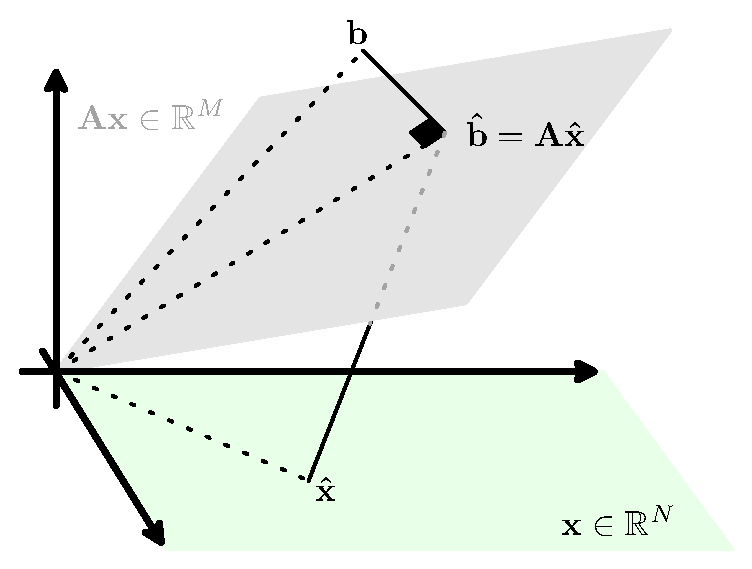
\includegraphics[width=0.9\textwidth]{chapters/minimization-fx/minimo-linear1.eps}
         \caption{Vetor $\VECTOR{d}_p$ perpendicular ao plano 
$\MATRIX{A}\VECTOR{x}$ traçado desde o ponto $\VECTOR{b}$. }
         \label{fig:coro:minAxbCAxb1:a}
     \end{figure}
\end{minipage}
\end{minipage}
\begin{minipage}{0.49\textwidth}
A partir do Teorema \ref{theo:minAxbCAxb}, 
podemos achar um vetor $\VECTOR{d}_p$ perpendicular ao plano $\MATRIX{A}\VECTOR{x}$,
partindo desde o ponto $\VECTOR{b}$, usando a seguinte equação,
\begin{equation}
\VECTOR{d}_p = \left\{\MATRIX{A}\left[ \MATRIX{A}^{\transpose}\MATRIX{A} \right]^{-1}\MATRIX{A}^{\transpose}- \MATRIX{I}\right\}\VECTOR{b},
\end{equation}
onde $I$ é uma matriz identidade.
Podemos ver graficamente o vetor $\VECTOR{d}_p$ na Figura \ref{fig:coro:minAxbCAxb1:a}.
%%
\index{Moore-Penrose!Pseudo-inversa}
\index{Pseudo-inversa!Moore-Penrose}
\begin{tcbattention}
A matriz $\left[ \MATRIX{A}^{\transpose}\MATRIX{A} \right]^{-1}\MATRIX{A}^{\transpose}$
também é chamada de pseudo inversa de Moore-Penrose da matriz $\MATRIX{A}$ \cite[pp. 290]{golub2013matrix}.
\end{tcbattention}
\end{minipage}
\end{corollary}

%%%%%%%%%%%%%%%%%%%%%%%%%%%%%%%%%%%%%%%%%%%%%%%%%%%%%%%%%%%%%%%%%%%%%%%%%%%%%%%%
\subsection{Exemplos de minimização de $||\MATRIX{A}\VECTOR{x}-\VECTOR{b}||_{\MATRIX{C}}^2$}

\begin{example}[Procurando um ponto 
$\VECTOR{\hat{x}}$ que minimize
 $||\MATRIX{A}\VECTOR{x}-\VECTOR{b}||_{\MATRIX{C}}^2$:]
\label{ex:minAxbCAxb1}
Conhecido 
um vetor coluna $\VECTOR{x}\in \mathbb{R}^2$,
as matrizes $\MATRIX{A} \in \mathbb{R}^{3\times 2}$ e $\MATRIX{C} \in \mathbb{R}^{3\times 3}_{+}$
e um ponto $\VECTOR{b} \in \mathbb{R}^{3}$,
achar o vetor $\VECTOR{x}$ que minimize $||\MATRIX{A}\VECTOR{x}-\VECTOR{b}||_{\MATRIX{C}}^2$;
sabendo que:
\begin{equation}
\VECTOR{b}=\begin{bmatrix}
1\\
1\\
1
\end{bmatrix},
\qquad 
\MATRIX{A}=\begin{bmatrix}
1 & 0\\
0 & 1\\
1 & 1
\end{bmatrix},
\qquad 
\MATRIX{C}=\begin{bmatrix}
1 & 0 & 0\\
0 & 1 & 0\\
0 & 0 & 1
\end{bmatrix}.
\end{equation}

Podemos ver a resposta a este exemplo na Solução \ref{ex:minAxbCAxb:sol1}.
\end{example}


\begin{SolutionT}[Relativa ao Exemplo \ref{ex:minAxbCAxb1}:]
\label{ex:minAxbCAxb:sol1}
Com todos estes dados e usando a Eq. (\ref{eq:minAxbCAxb1}),
obtemos a superfície $e(\VECTOR{x})$ como mostra a Figura \ref{fig:ex:minAxbCAxb:a}.
Usando a Eq. (\ref{eq:minAxbCAxb2}) sabemos que o ponto $\VECTOR{\hat{x}}=[1\quad 1]^{\transpose}$
minimiza a Eq. (\ref{eq:minAxbCAxb1}), com um $e(\VECTOR{\hat{x}})=0.12$.

Usando o Corolário \ref{coro:minAxbCAxb1}, podemos calcular o vetor $\VECTOR{d}_p=[0.2 \quad 0.2 \quad -0.2]^{\transpose}$,
como mostra o gráfico da Figura \ref{fig:ex:minAxbCAxb:b}.

\begin{figure}[h!]
     \centering
     \begin{subfigure}[b]{0.66\textwidth}
         \centering
         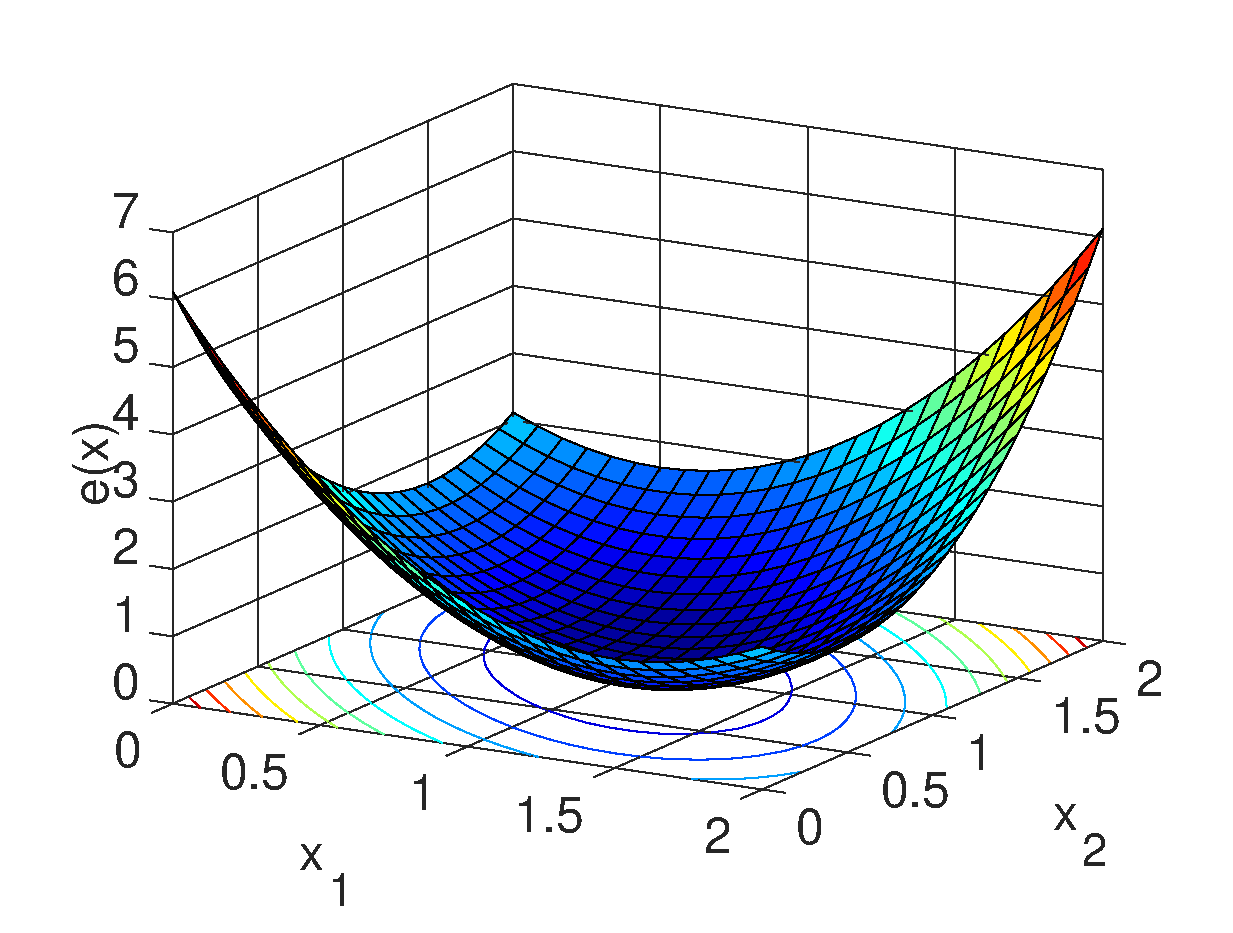
\includegraphics[width=0.98\textwidth]{chapters/minimization-fx/mfiles/ax1/surfcex.eps}
         \caption{Superfície $e(\VECTOR{x})$. }
         \label{fig:ex:minAxbCAxb:a}
     \end{subfigure}
     \hfill
     \begin{subfigure}[b]{0.32\textwidth}
         \centering
         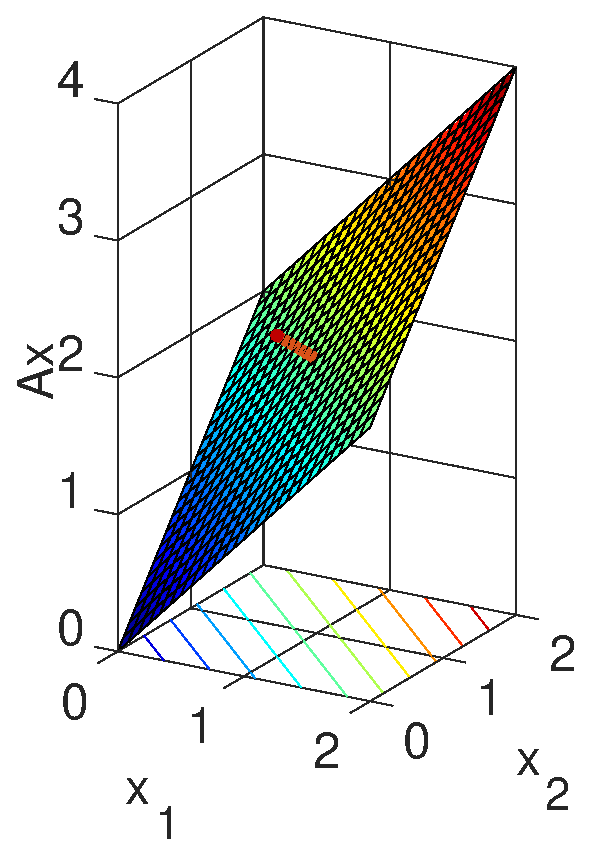
\includegraphics[width=0.98\textwidth]{chapters/minimization-fx/mfiles/ax1/surfcax.eps}
         \caption{Plano $\MATRIX{A}\VECTOR{x}$ e o vetor perpendicular $\VECTOR{b}-\MATRIX{A}\VECTOR{\hat{X}}$.}
         \label{fig:ex:minAxbCAxb:b}
     \end{subfigure}
        \caption{Resposta gráfica do Exemplo \ref{ex:minfxbCfxb3}. }
        \label{fig:ex:minAxbCAxb}
\end{figure}

\end{SolutionT}

\begin{comment}
\index{Tikhonov, Andrei Nikolaevich}
\begin{elaboracion}[title=Andrei Nikolaevich Tikhonov (1906-1993), width= 0.99\linewidth]
Matemático nascido em Rússia que trabalhou em distintas áreas como: 
topologia e análise funcional, 
equações diferenciais ordinárias e parciais, 
e sua aplicação a problemas em física matemática e matemática computacional \cite[pp. 3684]{ben2009historical}.
\end{elaboracion}
\end{comment}

\index{Tikhonov, Andrei Nikolaevich}
\index{Minimização, métodos!Regularização de Tikhonov}
\begin{tcbinformation} 
\textbf{Regularização de Tikhonov de ordem zero:} Este método foi trabalhado de forma independente
por Phillips em 1962 e por Andrei Nikolaevich Tikhonov em 1963 \cite[pp. 86]{kress2012numerical}, 
obtendo eles uma solução ótima para $\VECTOR{x}$  que minimiza $e(\VECTOR{x})$, 
\begin{equation}
e(\VECTOR{x})=||\MATRIX{A}\VECTOR{x}-\VECTOR{b}||^2+\alpha ||\VECTOR{x}||^2.
\end{equation}
Se no Teorema \ref{theo:minAxbCAxbplusalphaxqD} da  Seção \ref{sec:minAxbCAxbplusalphaxqD},
assumimos que o vetor $\VECTOR{q}=\VECTOR{0}$, a matriz $\MATRIX{C}=\MATRIX{I}$ e 
a matriz $\MATRIX{D}=\MATRIX{I}$,
então a solução representa a regularização de Tikhonov de ordem zero
\cite[pp. 94]{aster2013parameter} \cite[pp. 86]{kress2012numerical} \cite[pp. 117]{engl2000regularization}.
\end{tcbinformation} 

%%% high order tikhonov regularization \cite[pp. 103]{aster2013parameter}

\newpage

\section{Minimização de $||\MATRIX{A}\VECTOR{x}-\VECTOR{b}||_{\MATRIX{C}}^2+\alpha ||\VECTOR{x}-\VECTOR{q}||_{\MATRIX{D}}^2$
}

\begin{theorem}\label{theo:minAxbCAxbplusalphaxqD}
Dados,
o escalar $\alpha \in \mathbb{R}$, 
os vetores coluna $\VECTOR{x}\in \mathbb{R}^N$, 
$\VECTOR{b}\in \mathbb{R}^M$ e
$\VECTOR{q}\in \mathbb{R}^N$,  
uma matriz $\MATRIX{A} \in \mathbb{R}^{M\times N}$, 
as matrizes diagonais $\MATRIX{C} \in \mathbb{R}^{M\times M}$ e
$\MATRIX{D} \in \mathbb{R}^{N\times N}$, e 
definida a Eq. (\ref{eq:minAxbCAxb1alphaxqD}),
\begin{equation}\label{eq:minAxbCAxb1alphaxqD}
e(\VECTOR{x})  = ||\MATRIX{A}\VECTOR{x}-\VECTOR{b}||_{\MATRIX{C}}^2 +\alpha ||\VECTOR{x}-\VECTOR{q}||_{\MATRIX{D}}^2.
\end{equation}
Se desejamos ter o valor $\VECTOR{\hat{x}}$ que minimiza o escalar $e(\VECTOR{\hat{x}})$,
devemos usar\footnote{A demostração pode ser vista na Prova \ref{proof:theo:minAxbCAxbalphaxqD}.} a Eq. (\ref{eq:minAxbCAxb2alphaxqD}),
\begin{equation}\label{eq:minAxbCAxb2alphaxqD}
\VECTOR{\hat{x}}=\left[ \MATRIX{A}^{\transpose}\MATRIX{C}\MATRIX{A} +\alpha\MATRIX{D}\right]^{-1} 
\left[ \MATRIX{A}^{\transpose}\MATRIX{C} \VECTOR{b}+\alpha\MATRIX{D}\VECTOR{q}\right].
\end{equation}
Assim, o mínimo existe só sim $\MATRIX{A}^{\transpose}\MATRIX{C}\MATRIX{A} +\alpha\MATRIX{D}$ tem inversa.
\end{theorem}

\index{Pseudo-inversa de Moore-Penrose}
\index{Problema inverso!Linear}
\index{Minimização do erro quadrático!Linear}


\newpage

\section{Minimização de $||\VECTOR{f}(\VECTOR{x})-\VECTOR{b}||_{\MATRIX{C}}^2$}

%\index{Minimização, métodos!Regularização de }
%\index{Problema inverso!Não linear}
\index{Minimização do erro quadrático!Não linear}%!Função $||\VECTOR{f}(\VECTOR{x})-\VECTOR{b}||_{\MATRIX{C}}^2$}

\begin{theorem}[Solução iterativa:]\label{theo:minfxbCfxb}
Dados
os vetores coluna $\VECTOR{x}\in \mathbb{R}^N$ e $\VECTOR{b}\in \mathbb{R}^M$,  
uma função $\VECTOR{f}:\mathbb{R}^{N} \rightarrow \mathbb{R}^{M}$, 
uma matriz diagonal $\MATRIX{C} \in \mathbb{R}^{M\times M}_{+}$, e 
definida a Eq. (\ref{eq:minfxbCfxb1}),
\begin{equation}\label{eq:minfxbCfxb1}
\begin{matrix}
e(\VECTOR{x}) & = & ||\VECTOR{f}(\VECTOR{x})-\VECTOR{b}||_{\MATRIX{C}}^2 \\
              & = & (\VECTOR{f}(\VECTOR{x})-\VECTOR{b})^{\transpose}\MATRIX{C}(\VECTOR{f}(\VECTOR{x})-\VECTOR{b}).
\end{matrix}
\end{equation}
Se desejamos ter o ponto $\VECTOR{x}=\VECTOR{\hat{x}}$ que minimiza o escalar $e(\VECTOR{x})$,
podemos achar esse ponto usando iterativamente a Eq. (\ref{eq:minfxbCfxb2}),
em que $\MATRIX{J}(\VECTOR{x})$ é a \hyperref[def:jacobian]{\textbf{matriz Jacobiana}}  de $\VECTOR{f}(\VECTOR{x})$.
\begin{equation}\label{eq:minfxbCfxb2}
\VECTOR{x}_{k} \leftarrow \VECTOR{x}_{k-1}-
\left[ \MATRIX{J}(\VECTOR{x}_{k-1})^{\transpose}\MATRIX{C} \MATRIX{J}(\VECTOR{x}_{k-1}) \right]^{-1}
 \MATRIX{J}(\VECTOR{x}_{k-1})^{\transpose}\MATRIX{C}\left[\VECTOR{f}(\VECTOR{x}_{k-1})-\VECTOR{b}\right];
\end{equation}



Assim, $\VECTOR{\hat{x}}$ pode ser achado 
iniciando a Eq. (\ref{eq:minfxbCfxb2}) desde um $\VECTOR{x}_{0}$ qualquer, 
até que $\VECTOR{x}_{k}$ seja muito próximo a $\VECTOR{x}_{k-1}$,
em que se declara que $\VECTOR{\hat{x}} \approx \VECTOR{x}_{k}$,
que corresponde a um mínimo\footnote{\label{ref:minfx}A
demonstração pode ser vista na Prova \ref{proof:theo:minfxbCfxb}.} de $e(\VECTOR{x})$,
sem aclarar se é local ou global.

\textbf{Considerações:}

\begin{itemize}
\item Para que tenha sentido a Eq. (\ref{eq:minfxbCfxb2}),
 e consequentemente ela possa ser usada, devemos verificar que  $\MATRIX{J}(\VECTOR{x}_{k-1})\neq \MATRIX{0}$,
pois se $\MATRIX{J}(\VECTOR{x}_{k-1})= \MATRIX{0}$ indica que existe\footref{ref:minfx} um ponto de inflexão 
(máximo, mínimo ou ponto de sela) em $e(\VECTOR{x}_{k-1})$.
\item A busca iterativa da Eq. (\ref{eq:minfxbCfxb2}) é considerada falida quando 
$\MATRIX{J}(\VECTOR{x}_{k-1})^{\transpose}$ $\MATRIX{C}$ $\MATRIX{J}(\VECTOR{x}_{k-1})$
não tem inversa.
\item A busca iterativa da Eq. (\ref{eq:minfxbCfxb2}) pode divergir quando coincide que o mínimo $\VECTOR{\hat{x}}$ procurado
tem um $\MATRIX{J}(\VECTOR{\hat{x}})\approx \MATRIX{0}$.
O erro só acontece quando $\VECTOR{x}_{k-1}$ atinge de forma ``exata'' 
um mínimo com $\VECTOR{f}(\VECTOR{x}_{k-1})\neq \VECTOR{b}$;
para outros valores a busca iterativa de $\VECTOR{x}_{k-1}$ avança eficazmente.
\end{itemize}

\end{theorem}
%%%%%%%%%%%%%%%%%%%%%%%%%%%%%%%%%%%%%%%%%%%%%%%%%%%%%%%%%%%%%%%%%%%%%%%%%%%%%%%%
\subsection{Exemplos de minimização de $||\VECTOR{f}(\VECTOR{x})-\VECTOR{b}||_{\MATRIX{C}}^2$}

\begin{example}[Quando existe 
$\VECTOR{\hat{x}}$ que cumpre que $\VECTOR{f}(\VECTOR{\hat{x}}) \approx \VECTOR{b}$:]
\label{ex:minfxbCfxb}
Conhecida uma função $\VECTOR{f}(\VECTOR{x}) : \mathbb{R}^{2} \rightarrow \mathbb{R}^{3}$
e um ponto $\VECTOR{b}$ do contradomínio de $\VECTOR{f}(\VECTOR{x})$,
achar o valor $\VECTOR{\hat{x}}$ que minimize $||\VECTOR{f}(\VECTOR{x})-\VECTOR{b}||_{\MATRIX{C}}^2$;
sabendo que:
\begin{equation}
\VECTOR{b}=\begin{bmatrix}
1\\
1\\
2
\end{bmatrix},
\qquad 
\VECTOR{f}(\VECTOR{x})=\begin{bmatrix}
x_1^2\\
x_2^2\\
x_1+x_2
\end{bmatrix}.
\end{equation}
Consequentemente, podemos deduzir e escolher que, 
\begin{equation}\label{eq:lab:ex2fx}
\MATRIX{J}(\VECTOR{x})=\begin{bmatrix}
2 x_1 & 0\\
0 & 2 x_2\\
1 & 1
\end{bmatrix},
\qquad
\MATRIX{C}=\begin{bmatrix}
1 & 0 & 0\\
0 & 1 & 0\\
0 & 0 & 1
\end{bmatrix}.
\end{equation}
Com todos esses dados e usando a Eq. (\ref{eq:minfxbCfxb1}),
obtemos a superfície $e(\VECTOR{x})$ como mostra a Figura \ref{fig:ex:minfxbCfxb:a}.
Podemos ver as respostas a esse exemplo na Solução \ref{ex:minfxbCfxb:sol1} e \ref{ex:minfxbCfxb:sol2}.
\end{example}

\begin{SolutionT}[Relativa ao Exemplo \ref{ex:minfxbCfxb}:]
\label{ex:minfxbCfxb:sol1}
Se escolhemos o ponto inicial $\VECTOR{x}_0=[0.1~0.1]^{\transpose}$ e 
usamos iterativamente a Eq. (\ref{eq:minfxbCfxb2}), obtemos os valores 
de $\VECTOR{x}_k$ e $e(\VECTOR{x}_k)$, como mostra a Tabela \ref{table:ex:minfxbCfxb},
em que se asume o final do processo iterativo quando $\VECTOR{x}_k \approx \VECTOR{x}_{k-1}$.
Assim, a aproximação iterativa conclui na resposta $\VECTOR{\hat{x}}\approx \VECTOR{x}_{4} =[1~1]^{\transpose}$,
com um erro $e(\VECTOR{\hat{x}})=5.0032~10^{-24}\approx 0$ e uma pendente\footnote{\label{ref:pendenteex} O
cálculo da pendente de $e(\VECTOR{\hat{x}})$ pode ser visto no Teorema \ref{theo:derfxbCfxb0}.}
$\frac{\partial e(\VECTOR{\hat{x}})}{\partial \VECTOR{x} }=[7.7485~10^{-12}\quad 7.7485~10^{-12}]^{\transpose}$
próxima a zero;
esse processo pode ser visto de forma gráfica na Figura \ref{fig:ex:minfxbCfxb:b}.
\end{SolutionT}


\begin{table}[h!]
\centering
\begin{tabular}{|l|l|l|l|l|l|}
\hline
$k$ & 0 & 1 & 2 & 3 & 4 \\ \hline
$\VECTOR{x}_k$ & 0.10000   & 1.07941   & 1.00204   & 1.00000   & 1.00000 \\ 
~              & 0.10000   & 1.07941   & 1.00204   & 1.00000   & 1.00000 \\ \hline
$||\VECTOR{x}_k||$ & 0.14142   & 1.52652   & 1.41710   & 1.41421   & 1.41421 \\ \hline
$e(\VECTOR{x}_k)$ & 5.2002 &   7.9761e-02  & 5.0203e-05  & 2.3241e-11  & 5.0032e-24 \\ \hline
\end{tabular}
\caption{Resposta iterativa do Exemplo \ref{ex:minfxbCfxb}.}
\label{table:ex:minfxbCfxb}
\end{table}
\begin{figure}[h!]
     \centering
     \begin{subfigure}[b]{0.49\textwidth}
         \centering
         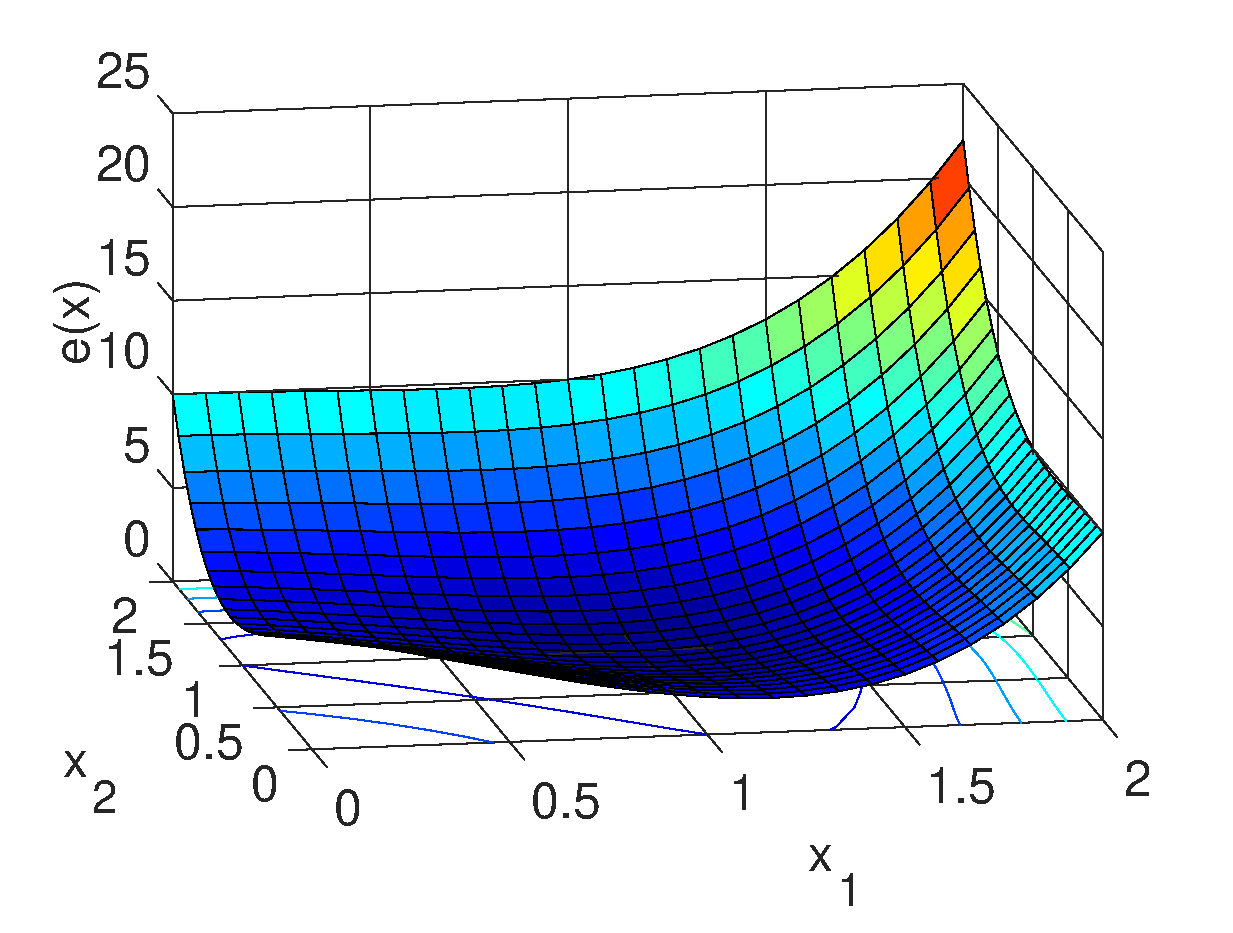
\includegraphics[width=0.98\textwidth]{chapters/minimization-fx/mfiles/fx1/surfcfx.eps}
         \caption{Superfície $e(\VECTOR{x})$. }
         \label{fig:ex:minfxbCfxb:a}
     \end{subfigure}
     \hfill
     \begin{subfigure}[b]{0.49\textwidth}
         \centering
         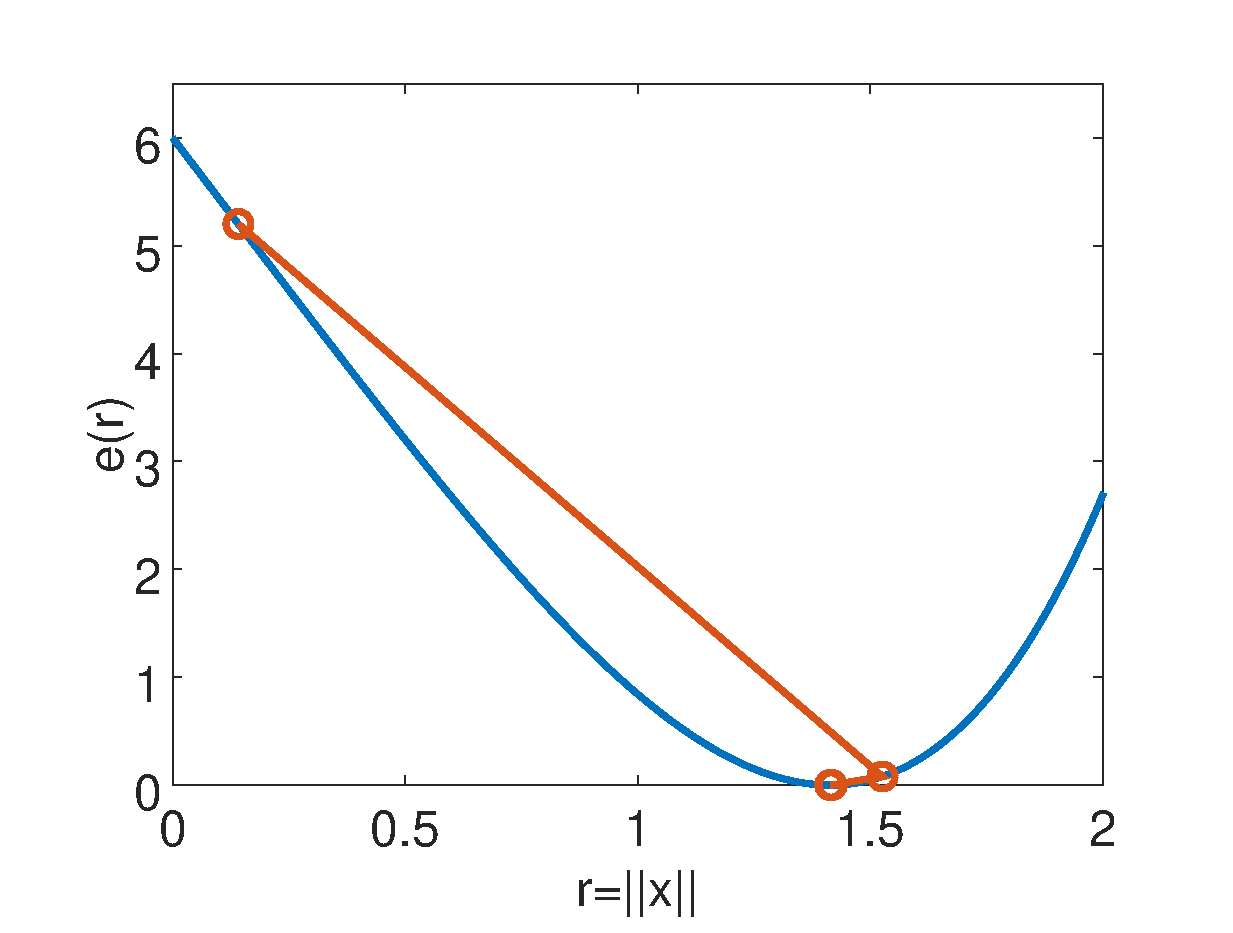
\includegraphics[width=0.98\textwidth]{chapters/minimization-fx/mfiles/fx1/plotfx.eps}
         \caption{Curva $e(\VECTOR{x})$ na direção $(1,1)$.}
         \label{fig:ex:minfxbCfxb:b}
     \end{subfigure}
        \caption{Resposta gráfica do Exemplo \ref{ex:minfxbCfxb}. }
        \label{fig:ex:minfxbCfxb}
\end{figure}


\begin{SolutionT}[Relativa ao Exemplo \ref{ex:minfxbCfxb}:]
\label{ex:minfxbCfxb:sol2}
É interessante resaltar que obteremos um erro,
se tentamos iniciar a busca iterativa desde a posição  $\VECTOR{x}_0=[0~0]^{\transpose}$
com pendente $\frac{\partial e(\VECTOR{x}_0)}{\partial \VECTOR{x} }=[-4~-4]^{\transpose}$,
pois a matriz $\MATRIX{J}(\VECTOR{x}_0)^{\transpose}\MATRIX{C} \MATRIX{J}(\VECTOR{x}_0)$
não tem inversa.
\end{SolutionT}


\begin{example}[Quando existe um
$\VECTOR{\hat{x}}$ que cumpre que $\VECTOR{f}(\VECTOR{\hat{x}}) \neq \VECTOR{b}$:]
\label{ex:minfxbCfxb2}
Conhecida uma função $\VECTOR{f}(\VECTOR{x}) : \mathbb{R}^{2} \rightarrow \mathbb{R}^{3}$
e um ponto $\VECTOR{b}$ que presumimos que existem no contradomínio $\VECTOR{f}(\VECTOR{x})$,
achar o valor $\VECTOR{\hat{x}}$ que minimize $||\VECTOR{f}(\VECTOR{x})-\VECTOR{b}||_{\MATRIX{C}}^2$;
sabendo que:
\begin{equation}
\VECTOR{b}=\begin{bmatrix}
1\\
1\\
1.5
\end{bmatrix},
\qquad 
\VECTOR{f}(\VECTOR{x})=\begin{bmatrix}
x_1^2\\
x_2^2\\
x_1+x_2
\end{bmatrix}.
\end{equation}
Com todos esses dados e usando a Eq. (\ref{eq:minfxbCfxb1}),
obtemos a superfície $e(\VECTOR{x})$ como mostra a Figura \ref{fig:ex:minfxbCfxb2:a},
na qual observamos que esta nunca atinge o valor zero.
Podemos ver uma resposta para este exemplo na Solução \ref{ex:minfxbCfxb2:sol1}.
\end{example}

\begin{SolutionT}[Relativa ao Exemplo \ref{ex:minfxbCfxb2}:]
\label{ex:minfxbCfxb2:sol1}
Este problema pode ser resolvido de forma similar ao Exemplo \ref{ex:minfxbCfxb},
usando os dados da Eq. (\ref{eq:lab:ex2fx}).
Assim, se escolhemos o ponto inicial $\VECTOR{x}_0=[0.1~0.1]^{\transpose}$ 
e usamos iterativamente a Eq. (\ref{eq:minfxbCfxb2}), obtemos os valores 
de $\VECTOR{x}_k$ e $e(\VECTOR{x}_k)$, como mostra a Tabela \ref{table:ex:minfxbCfxb2}.
A aproximação iterativa é feita até atingir $\VECTOR{x}_k \approx \VECTOR{x}_{k-1}$,
onde concluimos que a resposta é $\VECTOR{\hat{x}}\approx \VECTOR{x}_5 =[0.90856\quad 0.90856]^{\transpose}$
com um erro $e(\VECTOR{\hat{x}})=0.16148$; quer dizer, não existe $\VECTOR{f}(\VECTOR{\hat{x}})$
que seja igual a $\VECTOR{b}$, só podemos achar um vetor $\VECTOR{\hat{x}}$ 
que provoque um valor com mínimo erro, com pendente 
$\frac{\partial e(\VECTOR{\hat{x}})}{\partial \VECTOR{x} }=[-9.7332~10^{-6}\quad -9.7332~{10}^{-6}]^{\transpose}$
e um
\begin{equation}
\MATRIX{J}(\VECTOR{\hat{x}})=
\begin{bmatrix}
1.81712 & 0.0\\ 
0.0     & 1.81712\\
1       & 1
\end{bmatrix}.
\end{equation}
Todo esse processo pode ser visto de forma gráfica na Figura \ref{fig:ex:minfxbCfxb2:b}.
\end{SolutionT}

\begin{table}[h!]
\centering
\begin{tabular}{|l|l|l|l|l|l|l|}
\hline
$k$ & 0 & 1 & 2 & 3 & 4 & 5 \\ \hline
$\VECTOR{x}_k$ & 0.10000   & 0.83431   & 0.90507   & 0.90833   & 0.90855   & 0.90856 \\ 
~              & 0.10000   & 0.83431   & 0.90507   & 0.90833   & 0.90855   & 0.90856 \\ \hline
$||\VECTOR{x}_k||$ & 0.14142   & 1.17989   & 1.27996   & 1.28457   & 1.28488   & 1.28490 \\ \hline
$e(\VECTOR{x}_k)$ & 3.65020  & 0.21317  & 0.16160  & 0.16148  & 0.16148  & 0.16148 \\ \hline
\end{tabular}
\caption{Resposta iterativa do Exemplo \ref{ex:minfxbCfxb2}.}
\label{table:ex:minfxbCfxb2}
\end{table}
\begin{figure}[h!]
     \centering
     \begin{subfigure}[b]{0.49\textwidth}
         \centering
         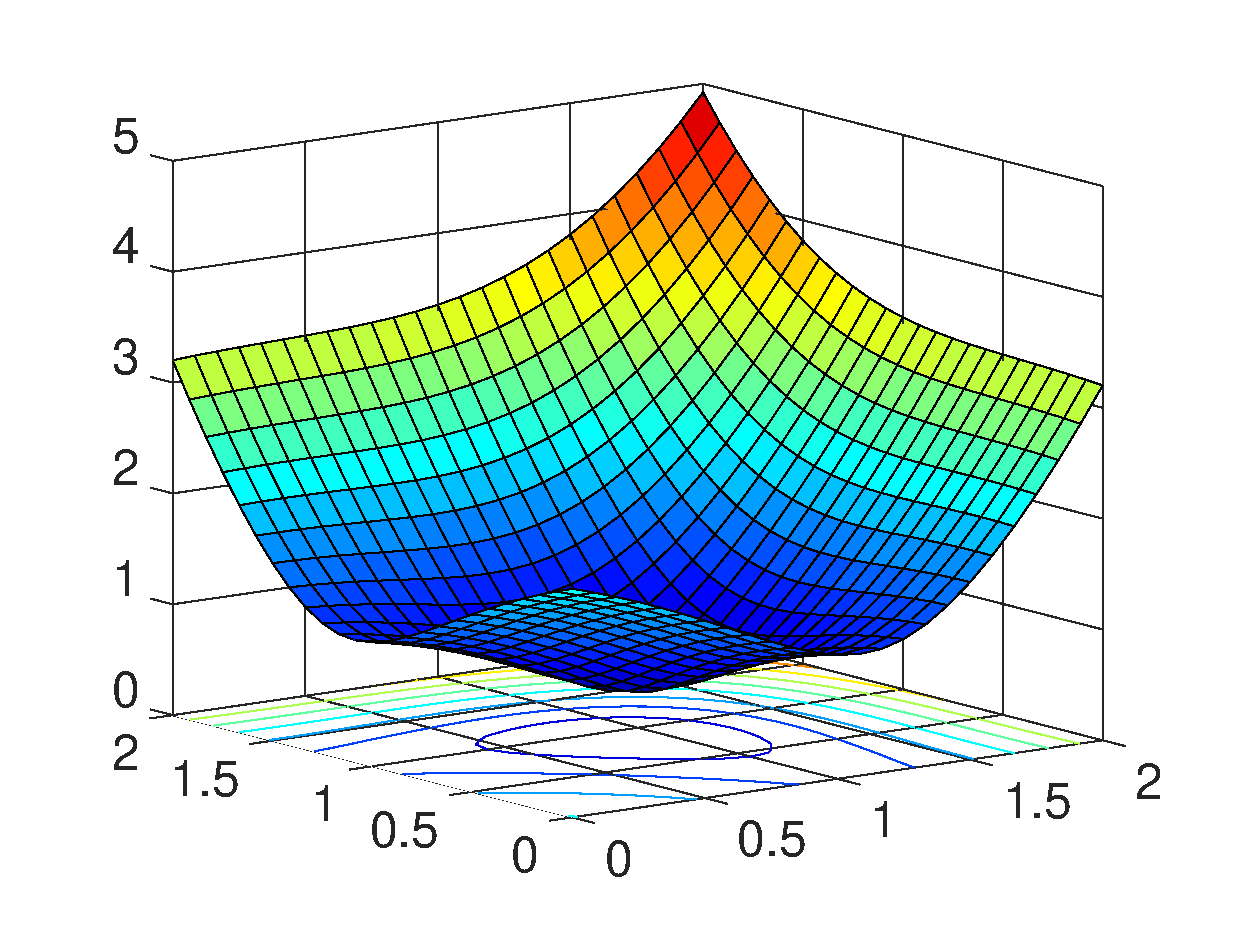
\includegraphics[width=0.98\textwidth]{chapters/minimization-fx/mfiles/fx1/surfcfx2.eps}
         \caption{Superfície $e(\VECTOR{x})$. }
         \label{fig:ex:minfxbCfxb2:a}
     \end{subfigure}
     \hfill
     \begin{subfigure}[b]{0.49\textwidth}
         \centering
         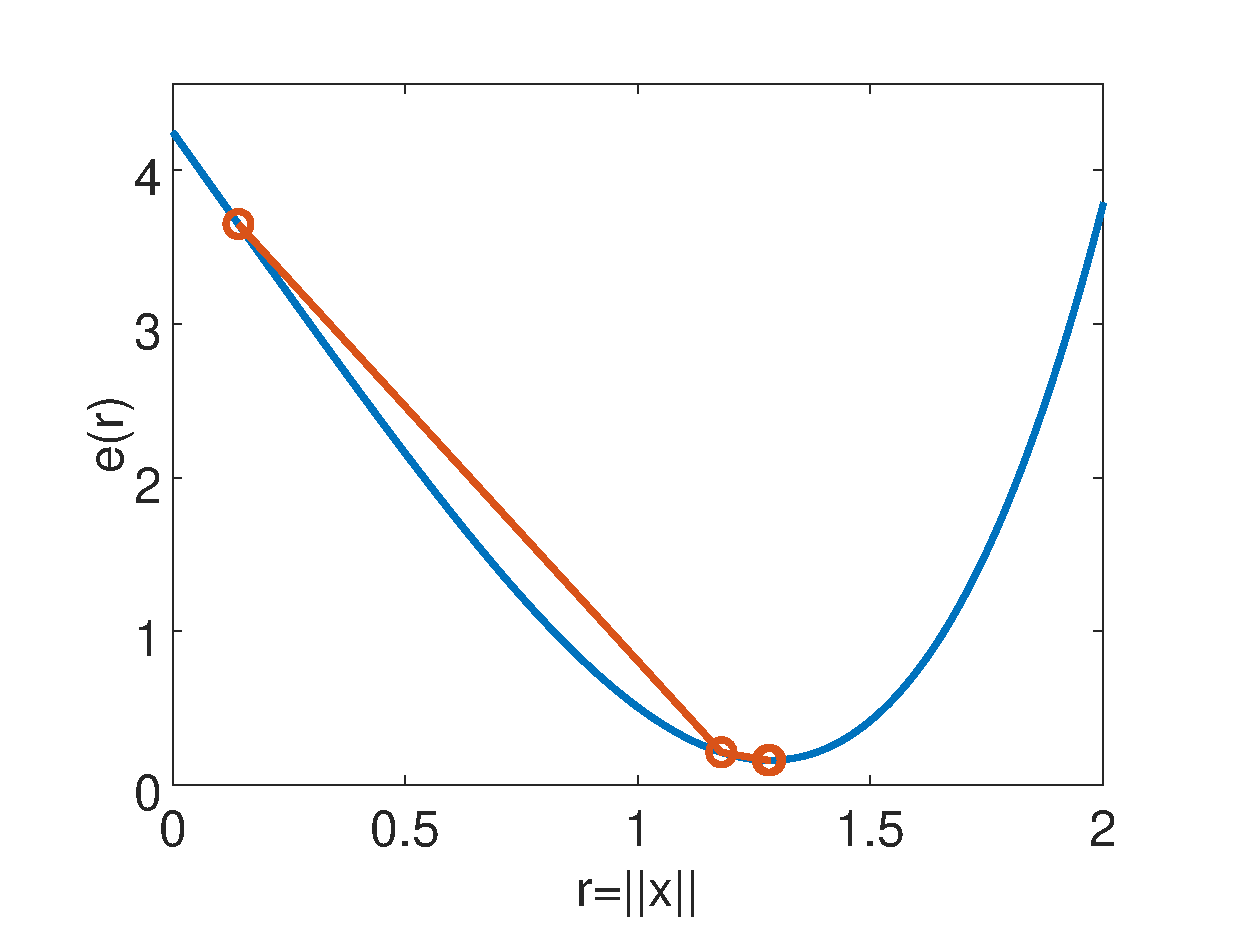
\includegraphics[width=0.98\textwidth]{chapters/minimization-fx/mfiles/fx1/plotfx2.eps}
         \caption{Curva $e(\VECTOR{x})$ na direção $(1,1)$.}
         \label{fig:ex:minfxbCfxb2:b}
     \end{subfigure}
        \caption{Resposta gráfica do Exemplo \ref{ex:minfxbCfxb2}. }
        \label{fig:ex:minfxbCfxb2}
\end{figure}


\begin{example}[Quando existem muitos mínimos locais e um
$\VECTOR{\hat{x}}$ que cumpre que $\VECTOR{f}(\VECTOR{\hat{x}}) \approx \VECTOR{b}$:]
\label{ex:minfxbCfxb3}
Conhecidos uma função $\VECTOR{f}(\VECTOR{x}) : \mathbb{R}^{2} \rightarrow \mathbb{R}^{3}$
e um ponto $\VECTOR{b}$ do contradomínio de $\VECTOR{f}(\VECTOR{x})$,
achar o valor $\VECTOR{\hat{x}}$ que minimize $||\VECTOR{f}(\VECTOR{x})-\VECTOR{b}||_{\MATRIX{C}}^2$;
sabendo que:
\begin{equation}
\VECTOR{b}=\begin{bmatrix}
1\\
1\\
2
\end{bmatrix},
\qquad 
\VECTOR{f}(\VECTOR{x})=\begin{bmatrix}
sin(\frac{x_1 5 \pi}{2})\\
sin(\frac{x_2 5 \pi}{2})\\
x_1+x_2
\end{bmatrix}.
\end{equation}
Consequentemente, podemos deduzir e escolher que, 
\begin{equation}\label{eq:lab:ex2fx3}
\MATRIX{J}(\VECTOR{x})=\begin{bmatrix}
\frac{5 \pi}{2}cos(\frac{x_1 5 \pi}{2}) & 0\\
0 & \frac{5 \pi}{2}cos(\frac{x_2 5 \pi}{2}) \\
1 & 1
\end{bmatrix},
\qquad
\MATRIX{C}=\begin{bmatrix}
1 & 0 & 0\\
0 & 1 & 0\\
0 & 0 & 1
\end{bmatrix}.
\end{equation}
Com todos esses dados e usando a Eq. (\ref{eq:minfxbCfxb1}),
obtemos a superfície $e(\VECTOR{x})$ como mostra a Figura \ref{fig:ex:minfxbCfxb3:a}.
Podemos ver as respostas a este exemplo na Solução \ref{ex:minfxbCfxb3:sol1} e \ref{ex:minfxbCfxb3:sol2}.
\end{example}

\begin{SolutionT}[Relativa ao Exemplo \ref{ex:minfxbCfxb3}:]
\label{ex:minfxbCfxb3:sol1}
Se escolhemos o ponto inicial $\VECTOR{x}_0=[\frac{11.0999}{5}$ $\frac{11.0999}{5}]^{\transpose}$,
com pendente\footnote{O cálculo da
pendente de $e(\VECTOR{\hat{x}})$ pode ser visto no Teorema \ref{theo:derfxbCfxb0}.} 
$\frac{\partial e(\VECTOR{x}_0)}{\partial \VECTOR{x} }=[4.2318~10^{-4}\quad 4.2318~10^{-4}]^{\transpose}$ e 
usamos iterativamente a Eq. (\ref{eq:minfxbCfxb2}), obtemos os valores 
de $\VECTOR{x}_k$ e $e(\VECTOR{x}_k)$, como mostra a Tabela \ref{table:ex:minfxbCfxb3},
onde se asume o final do processo iterativo quando $\VECTOR{x}_k \approx \VECTOR{x}_{k-1}$.
Assim, a aproximação iterativa conclui na resposta $\VECTOR{\hat{x}}\approx \VECTOR{x}_{7} =[1.7076\quad 1.7076]^{\transpose}$
com um erro $e(\VECTOR{\hat{x}})=2.1298$, uma pendente
$\frac{\partial e(\VECTOR{\hat{x}})}{\partial \VECTOR{x} }=[0.20251\quad 0.20251]^{\transpose}$
e um
\begin{equation}
\MATRIX{J}(\VECTOR{\hat{x}})=
\begin{bmatrix}
5.21306 & 0.0\\ 
0.0     & 5.21306\\
1       & 1
\end{bmatrix};
\end{equation}
esse processo pode ser visto de forma gráfica na Figura \ref{fig:ex:minfxbCfxb3:b}.

É interesante resaltar que o ponto $\VECTOR{x}_0$ é muito próximo a um máximo local de 
$e(\VECTOR{x})$, e o uso iterativo da Eq. (\ref{eq:minfxbCfxb2}) 
provoca o afastamento desse ponto, mesmo que a princípio os passos sejam pequenos;
por outro lado, a busca iterativa converge e finaliza em $\VECTOR{x}_7$ um mínimo local 
de $e(\VECTOR{x})$.

\end{SolutionT}

\begin{table}[h!]
\centering
\begin{tabular}{|l|l|l|l|l|l|l|l|l|}
\hline
$k$ & 0 & 1 & 2 & 3 & 4 & 5 & 6 & 7\\ \hline
$\VECTOR{x}_k$ & 2.2200   & 2.2199   & 2.2178   & 2.1385   & 1.5400   & 1.7184   & 1.6974   & 1.7076 \\ 
~              & 2.2200   & 2.2199   & 2.2178   & 2.1385   & 1.5400   & 1.7184   & 1.6974   & 1.7076 \\ \hline
$||\VECTOR{x}_k||$ & 3.1396   & 3.1394   & 3.1364   & 3.0243   & 2.1779   & 2.4302   & 2.4005   & 2.4149 \\ \hline
$e(\VECTOR{x}_k)$ & 13.8554  & 13.8554  & 13.8543  & 12.2971   & 5.3932   & 2.1432   & 2.1346   & 2.1298 \\ \hline
\end{tabular}
\caption{Resposta iterativa do Exemplo \ref{ex:minfxbCfxb3}.}
\label{table:ex:minfxbCfxb3}
\end{table}
\begin{figure}[h!]
     \centering
     \begin{subfigure}[b]{0.49\textwidth}
         \centering
         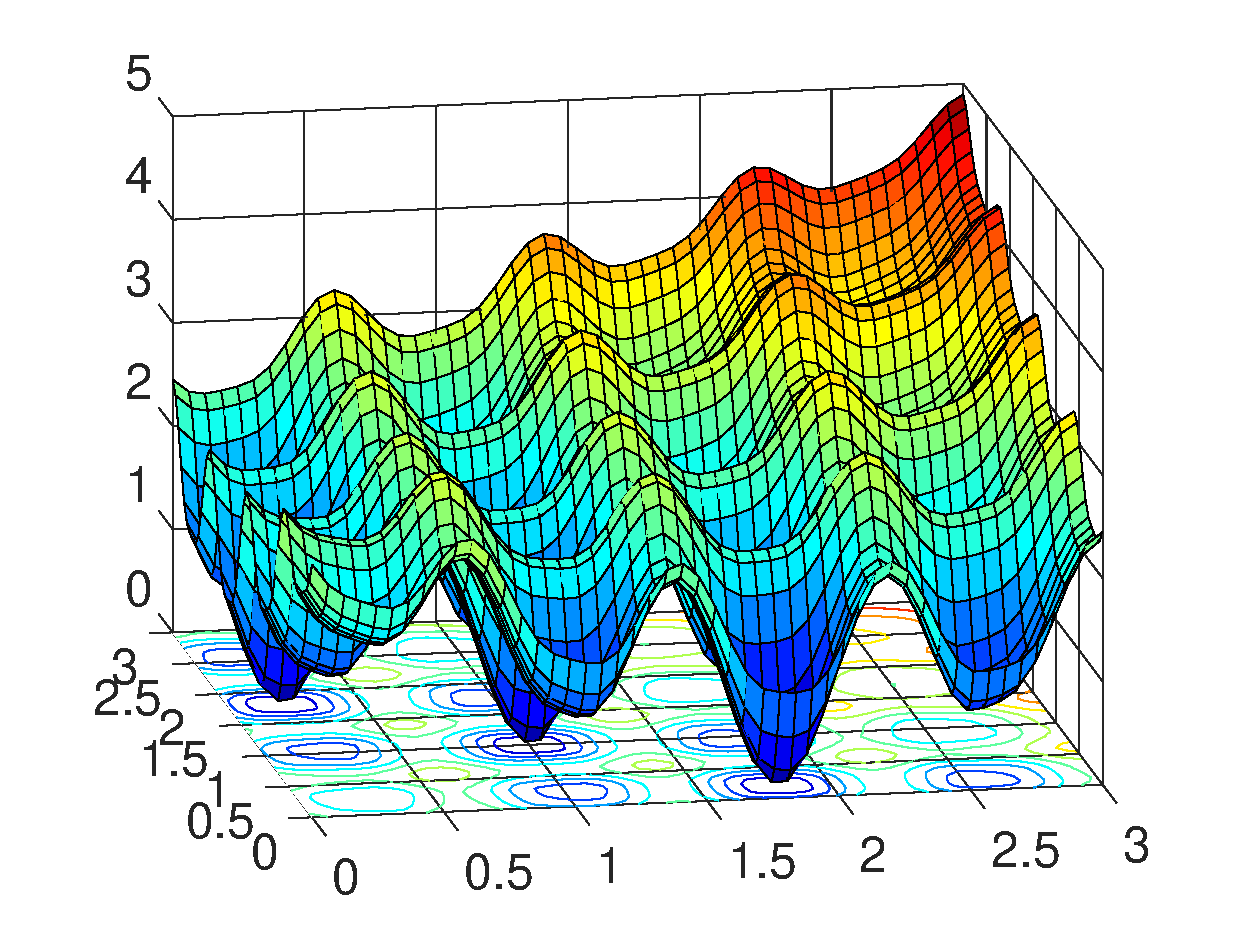
\includegraphics[width=0.98\textwidth]{chapters/minimization-fx/mfiles/fx3/surfcfx3.eps}
         \caption{Superfície $e(\VECTOR{x})$. }
         \label{fig:ex:minfxbCfxb3:a}
     \end{subfigure}
     \hfill
     \begin{subfigure}[b]{0.49\textwidth}
         \centering
         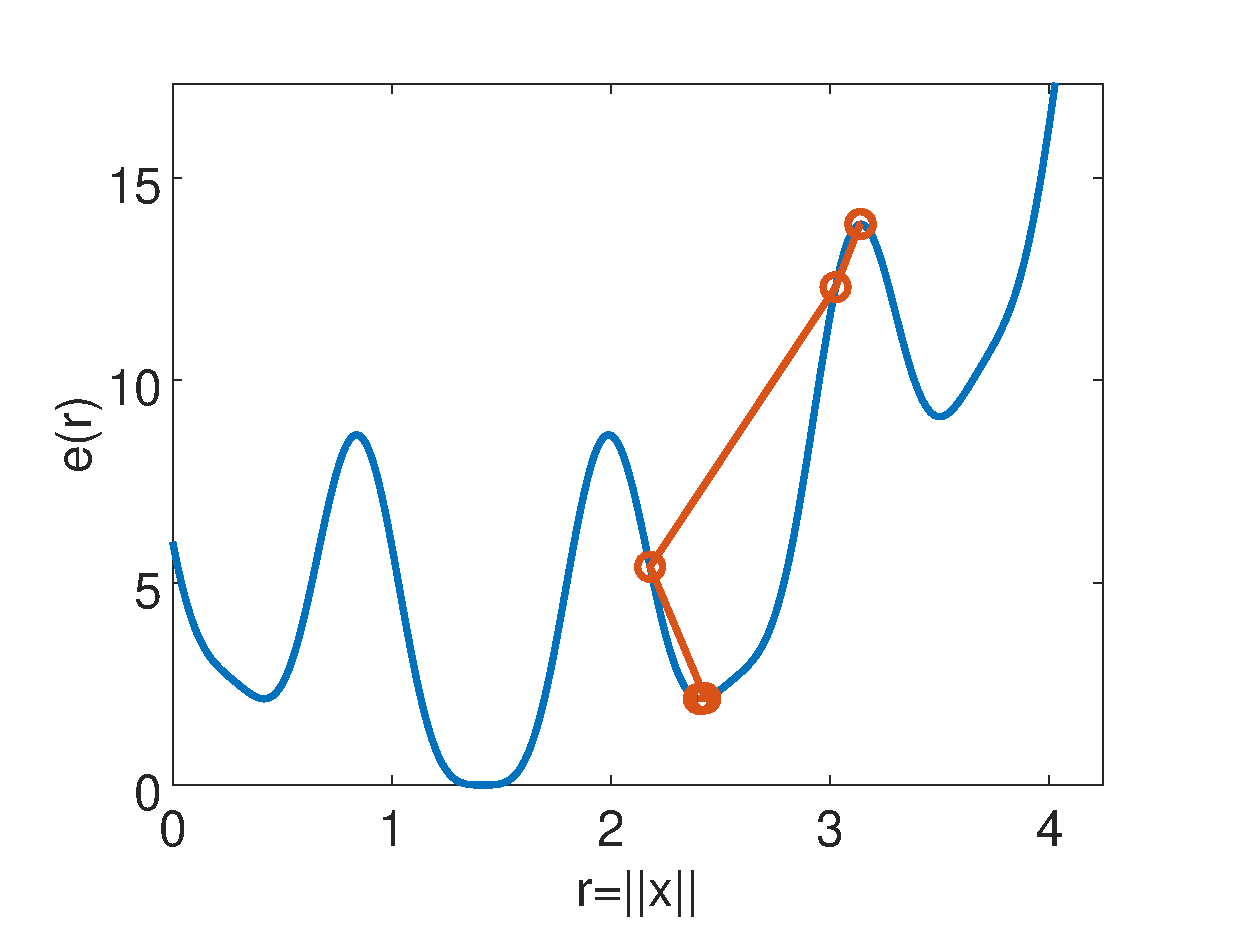
\includegraphics[width=0.98\textwidth]{chapters/minimization-fx/mfiles/fx3/plotfx3.eps}
         \caption{Curva $e(\VECTOR{x})$ na direção $(1,1)$.}
         \label{fig:ex:minfxbCfxb3:b}
     \end{subfigure}
        \caption{Resposta gráfica do Exemplo \ref{ex:minfxbCfxb3}. }
        \label{fig:ex:minfxbCfxb3}
\end{figure}

\begin{SolutionT}[Relativa ao Exemplo \ref{ex:minfxbCfxb3}:]
\label{ex:minfxbCfxb3:sol2}
Se escolhemos o ponto inicial $\VECTOR{x}_0=[\frac{7.032993}{5}$ $\frac{7.032993}{5}]^{\transpose}$,
com pendente\footnote{O cálculo da
pendente de $e(\VECTOR{\hat{x}})$ pode ser visto no Teorema \ref{theo:derfxbCfxb0}.} 
$\frac{\partial e(\VECTOR{x}_0)}{\partial \VECTOR{x} }=[7.6342~10^{-5}\quad 7.6342~10^{-5}]^{\transpose}$ e 
usamos iterativamente a Eq. (\ref{eq:minfxbCfxb2}), obtemos os valores 
de $\VECTOR{x}_k$ e $e(\VECTOR{x}_k)$, como mostra a Tabela \ref{table:ex:minfxbCfxb4},
em que se asume o final do processo iterativo quando $\VECTOR{x}_k \approx \VECTOR{x}_{k-1}$.
Assim, a aproximação iterativa conclui na resposta $\VECTOR{\hat{x}}\approx \VECTOR{x}_{7} =[0.99056\quad 0.99056]^{\transpose}$,
com um erro $e(\VECTOR{\hat{x}})=3.7152~10^{-4}$, uma pendente
$\frac{\partial e(\VECTOR{\hat{x}})}{\partial \VECTOR{x} }=[-0.040955\quad -0.040955]^{\transpose}$
e um
\begin{equation}
\MATRIX{J}(\VECTOR{\hat{x}})=
\begin{bmatrix}
0.58175 & 0.0\\ 
0.0     & 0.58175\\
1       & 1
\end{bmatrix};
\end{equation}
esse processo pode ser visto de forma gráfica na Figura \ref{fig:ex:minfxbCfxb4:b}.

De forma similar ao Exemplo \ref{ex:minfxbCfxb3:sol1}, observamos 
que o ponto $\VECTOR{x}_0$ é muito próximo a um máximo local de 
$e(\VECTOR{x})$, e o uso iterativo da Eq. (\ref{eq:minfxbCfxb2}) 
provoca o afastamento desse ponto, mesmo que a princípio os passos sejam pequenos;
por outro lado, a busca iterativa converge e finaliza em $\VECTOR{x}_7$ um mínimo global
de $e(\VECTOR{x})$.
\end{SolutionT}


\begin{table}[h!]
\centering
\begin{tabular}{|l|l|l|l|l|l|l|l|l|}
\hline
$k$ & 0 & 1 & 2 & 3 & 4 & 5 & 6 & 7\\ \hline
$\VECTOR{x}_k$ & 1.40660   & 1.40658   & 1.40558   & 1.34728   & 0.78432   & 0.93066   & 0.96985   & 0.99056 \\ 
~              & 1.40660   & 1.40658   & 1.40558   & 1.34728   & 0.78432   & 0.93066   & 0.96985   & 0.99056 \\ \hline
$||\VECTOR{x}_k||$ & 1.9892   & 1.9892   & 1.9878   & 1.9053   & 1.1092   & 1.3162   & 1.3716   & 1.4009 \\ \hline
$e(\VECTOR{x}_k)$ & 8.6506  & 8.6506  & 8.6503  & 7.8206  & 2.7076  & 6.109e-2 &  5.192e-3  & 3.715e-4 \\ \hline
\end{tabular}
\caption{Resposta iterativa do Exemplo \ref{ex:minfxbCfxb3}.}
\label{table:ex:minfxbCfxb4}
\end{table}

     \begin{figure}[!h]
         \centering
         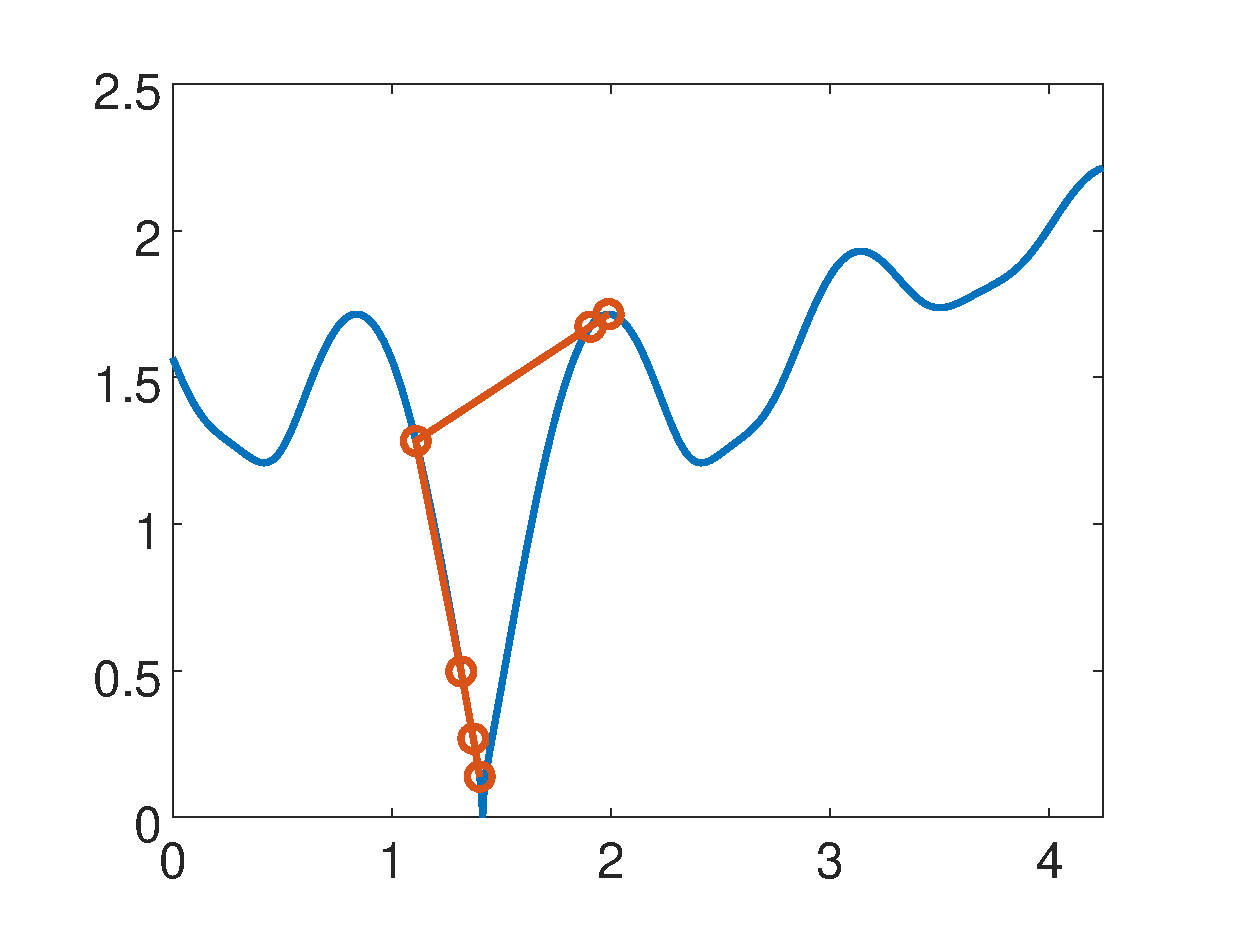
\includegraphics[width=0.5\textwidth]{chapters/minimization-fx/mfiles/fx3/plotfx4.eps}
         \caption{Curva $e(\VECTOR{x})$ na direção $(1,1)$.}
         \label{fig:ex:minfxbCfxb4:b}
     \end{figure}



\newpage

\section{Minimização de $||\VECTOR{f}(\VECTOR{x})-\VECTOR{b}||_{\MATRIX{C}}^2+\alpha||\VECTOR{x}-\VECTOR{q}||_{\MATRIX{D}}^2$}


%\index{Minimização, métodos!Regularização de }
%\index{Problema inverso!Não linear}
\index{Minimização do erro quadrático!Não linear}%!Função $||\VECTOR{f}(\VECTOR{x})-\VECTOR{b}||_{\MATRIX{C}}^2+\alpha||\VECTOR{x}-\VECTOR{q}||_{\MATRIX{D}}^2$}

\begin{theorem}[Solução iterativa:]\label{theo:minfxbCfxbaxqaxq}
Dados
o escalar $\alpha \in \mathbb{R}_{+}$,
os vetores coluna $\VECTOR{x}\in \mathbb{R}^N$, $\VECTOR{b}\in \mathbb{R}^M$ e $\VECTOR{q}\in \mathbb{R}^N$,  
uma função $\VECTOR{f}:\mathbb{R}^{N} \rightarrow \mathbb{R}^{M}$, 
as matrizes diagonais $\MATRIX{C} \in \mathbb{R}^{M\times M}_{+}$ e $\MATRIX{D} \in \mathbb{R}^{N\times N}_{+}$, e 
definida a Eq. (\ref{eq:minfxbCfxbaxqaxq1}),
\begin{align}\label{eq:minfxbCfxbaxqaxq1}
e(\VECTOR{x}) &=||\VECTOR{f}(\VECTOR{x})-\VECTOR{b}||_{\MATRIX{C}}^2+\alpha||\VECTOR{x}-\VECTOR{q}||_{\MATRIX{D}}^2\\
              & = (\VECTOR{f}(\VECTOR{x})-\VECTOR{b})^{\transpose}\MATRIX{C}(\VECTOR{f}(\VECTOR{x})-\VECTOR{b})+\alpha(\VECTOR{x}-\VECTOR{q})^{\transpose}\MATRIX{D}(\VECTOR{x}-\VECTOR{q}).
\end{align}
Se desejamos ter o ponto $\VECTOR{x}=\VECTOR{\hat{x}}$, que minimiza o escalar $e(\VECTOR{x})$,
podemos achar esse ponto usando iterativamente a Eq. (\ref{eq:minfxbCfxbaxqaxq2}),
em que $\MATRIX{J}(\VECTOR{x})$ é a \hyperref[def:jacobian]{\textbf{matriz Jacobiana}}  de $\VECTOR{f}(\VECTOR{x})$,
\begin{equation}\label{eq:minfxbCfxbaxqaxq2}
\VECTOR{x}_{k}\leftarrow \VECTOR{x}_{k-1}-
\left[ \MATRIX{J}(\VECTOR{x}_{k-1})^{\transpose}\MATRIX{C} \MATRIX{J}(\VECTOR{x}_{k-1}) +\alpha\MATRIX{D} \right]^{-1}
 \left\{\MATRIX{J}(\VECTOR{x}_{k-1})^{\transpose}\MATRIX{C}\left[\VECTOR{f}(\VECTOR{x}_{k-1})-\VECTOR{b}\right]+\alpha\MATRIX{D}\left[\VECTOR{x}_{k-1}-\VECTOR{q}\right]\right\},
\end{equation}

Assim, $\VECTOR{\hat{x}}$ pode ser achado 
iniciando a Eq. (\ref{eq:minfxbCfxbaxqaxq2}) desde um $\VECTOR{x}_{0}$ qualquer, 
até que $\VECTOR{x}_{k}$ seja muito próximo a $\VECTOR{x}_{k-1}$,
nesse caso declaramos que $\VECTOR{\hat{x}} \approx \VECTOR{x}_{k}$,
que corresponde a um mínimo\footnote{\label{ref:minfxxq}A
demonstração pode ser vista na Prova \ref{proof:theo:minfxbCfxbaxqd}.} de $e(\VECTOR{x})$,
sem esclarecer se é local ou global.


\textbf{Considerações:}

\begin{itemize}
\item É interessante verificar na Eq. (\ref{eq:minfxbCfxbaxqaxq2}) 
se  $\MATRIX{J}(\VECTOR{x}_{k-1}=\VECTOR{q}) = \MATRIX{0}$,
pois indica que existe\footref{ref:minfxxq} um ponto de inflexão 
(máximo, mínimo ou ponto de sela) em $e(\VECTOR{x}_{k-1}=\VECTOR{q})$;
consequentemente, poderíamos ter achado um mínimo\footnote{\label{foot:labq}É 
interessante verificar o ponto $\VECTOR{q}$, uma vez só, 
antes de iniciar a busca iterativa.}.
\item A busca iterativa da Eq. (\ref{eq:minfxbCfxbaxqaxq2}) falha quando 
$\MATRIX{J}(\VECTOR{x}_{k-1})^{\transpose}\MATRIX{C} \MATRIX{J}(\VECTOR{x}_{k-1}) +\alpha\MATRIX{D}$
não tem inversa.
\end{itemize}

\end{theorem} 

\begin{tcbattention}
\begin{itemize}
\item O Teorema \ref{theo:minfxbCfxbaxqaxq} pode ser usado para achar o vetor $\VECTOR{x}$
que minimize $e(\VECTOR{x})=||\VECTOR{f}(\VECTOR{x})-\VECTOR{b}||_{\MATRIX{C}}^2+\alpha||\VECTOR{x}-\VECTOR{q}||_{\MATRIX{D}}^2$,
quando sabemos que o vetor $\VECTOR{x}$ que minimiza $||\VECTOR{f}(\VECTOR{x})-\VECTOR{b}||_{\MATRIX{C}}^2$ 
está perto do ponto $\VECTOR{q}$.
\item No Teorema \ref{theo:minfxbCfxbaxqaxq}, o vetor $\VECTOR{x}$ que minimiza $e(\VECTOR{x})$ 
não necessariamente minimiza  $||\VECTOR{f}(\VECTOR{x})-\VECTOR{b}||_{\MATRIX{C}}^2$.
\end{itemize}
\end{tcbattention}

%%%%%%%%%%%%%%%%%%%%%%%%%%%%%%%%%%%%%%%%%%%%%%%%%%%%%%%%%%%%%%%%%%%%%%%%%%%%%%%%
\subsection{Exemplos de minimização de 
$||\VECTOR{f}(\VECTOR{x})-\VECTOR{b}||_{\MATRIX{C}}^2+\alpha||\VECTOR{x}-\VECTOR{q}||_{\MATRIX{D}}^2$}


\begin{example}[Quando existem muitos mínimos locais e um
$\VECTOR{\hat{x}}$ que cumpre que $\VECTOR{f}(\VECTOR{\hat{x}}) \approx \VECTOR{b}$:]
\label{ex:minfxbCfxbaxqaxq1}
Conhecidos um escalar $\alpha$, uma função $\VECTOR{f}(\VECTOR{x}) : \mathbb{R}^{2} \rightarrow \mathbb{R}^{3}$,
um ponto $\VECTOR{q}$
e outro ponto $\VECTOR{b}$, no domínio e no contradomínio de $\VECTOR{f}(\VECTOR{x})$, respetivamente;
achar o valor $\VECTOR{\hat{x}}$ que minimize 
$||\VECTOR{f}(\VECTOR{x})-\VECTOR{b}||_{\MATRIX{C}}^2+\alpha||\VECTOR{x}-\VECTOR{q}||_{\MATRIX{D}}^2$;
sabendo que:
\begin{equation}
\VECTOR{b}=\begin{bmatrix}
1\\
1\\
2
\end{bmatrix},
\qquad 
\VECTOR{f}(\VECTOR{x})=\begin{bmatrix}
sin(\frac{x_1 5 \pi}{2})\\
sin(\frac{x_2 5 \pi}{2})\\
x_1+x_2
\end{bmatrix},
\qquad
\alpha=0.1,
\qquad
\VECTOR{q}=\begin{bmatrix}
0\\
0\\
0
\end{bmatrix}.
\end{equation}
Com essa informação, podemos calcular o jacobiano $\MATRIX{J}(\VECTOR{x})$ de $\VECTOR{f}(\VECTOR{x})$,
 e escolher as matrizes $\MATRIX{C} \in \mathbb{R}^{3\times 3}_{+}$ e $\MATRIX{D} \in \mathbb{R}^{2\times 2}_{+}$, 
com elementos iguais à  matriz identidade. 
Assim, usando a Eq. (\ref{eq:minfxbCfxbaxqaxq1}),
obtemos a superfície $e(\VECTOR{x})$ como mostra a Figura \ref{fig:ex:minfxbCfxbaxqaxq3:a}.
Podemos ver duas respostas a este exemplo na Solução \ref{ex:minfxbCfxbaxqaxq3:sol1} e \ref{ex:minfxbCfxbaxqaxq3:sol2}.
\end{example}

\begin{SolutionT}[Relativa ao Exemplo \ref{ex:minfxbCfxbaxqaxq1}:]
\label{ex:minfxbCfxbaxqaxq3:sol1}
Se escolhemos o ponto inicial $\VECTOR{x}_0=[2\quad 2]^{\transpose}$,
com pendente\footnote{O cálculo da
pendente de $e(\VECTOR{\hat{x}})$ pode ser visto no Teorema \ref{theo:derfxbCfxb0}.} 
$\frac{\partial e(\VECTOR{x}_0)}{\partial \VECTOR{x} }=[20.108\quad 20.108]^{\transpose}$ e 
usamos iterativamente a Eq. (\ref{eq:minfxbCfxbaxqaxq2}), obtemos os valores 
$\VECTOR{x}_k$ e $e(\VECTOR{x}_k)$, como mostra a Tabela \ref{table:ex:minfxbCfxbaxqaxq3},
na qual se assume o final do processo iterativo quando $\VECTOR{x}_k \approx \VECTOR{x}_{k-1}$.
Assim, a aproximação iterativa conclui na resposta 
$\VECTOR{\hat{x}}\approx \VECTOR{x}_{7} =[1.7013\quad 1.7013]^{\transpose}$
com um erro $e(\VECTOR{\hat{x}})=2.7094$ e uma pendente
$\frac{\partial e(\VECTOR{\hat{x}})}{\partial \VECTOR{x} }=[0.0016997\quad 0.0016997]^{\transpose}$;
esse processo pode ser visto de forma gráfica na Figura \ref{fig:ex:minfxbCfxbaxqaxq3:b}.
\end{SolutionT}

\begin{table}[h!]
\centering
\begin{tabular}{|l|l|l|l|l|l|l|l|l|}
\hline
$k$ & 0 & 1 & 2 & 3 & 4 & 5 & 6 & 7\\ \hline
$\VECTOR{x}_k$ & 2.0000 & 1.8424 & 1.6110 & 1.7021 & 1.7009 & 1.7014 & 1.7012 & 1.7013 \\ 
~              & 2.0000 & 1.8424 & 1.6110 & 1.7021 & 1.7009 & 1.7014 & 1.7012 & 1.7013 \\ \hline
$||\VECTOR{x}_k||$ & 2.8284 & 2.6055 & 2.2782 & 2.4071 & 2.4055 & 2.4061 & 2.4059 & 2.4060 \\ \hline
$e(\VECTOR{x}_k)$ & 6.8000 & 3.5233 & 3.6832 & 2.7095 & 2.7094 & 2.7094 & 2.7094 & 2.7094 \\ \hline
\end{tabular}
\caption{Resposta iterativa do Exemplo \ref{ex:minfxbCfxbaxqaxq1}.}
\label{table:ex:minfxbCfxbaxqaxq3}
\end{table}
\begin{figure}[h!]
     \centering
     \begin{subfigure}[b]{0.49\textwidth}
         \centering
         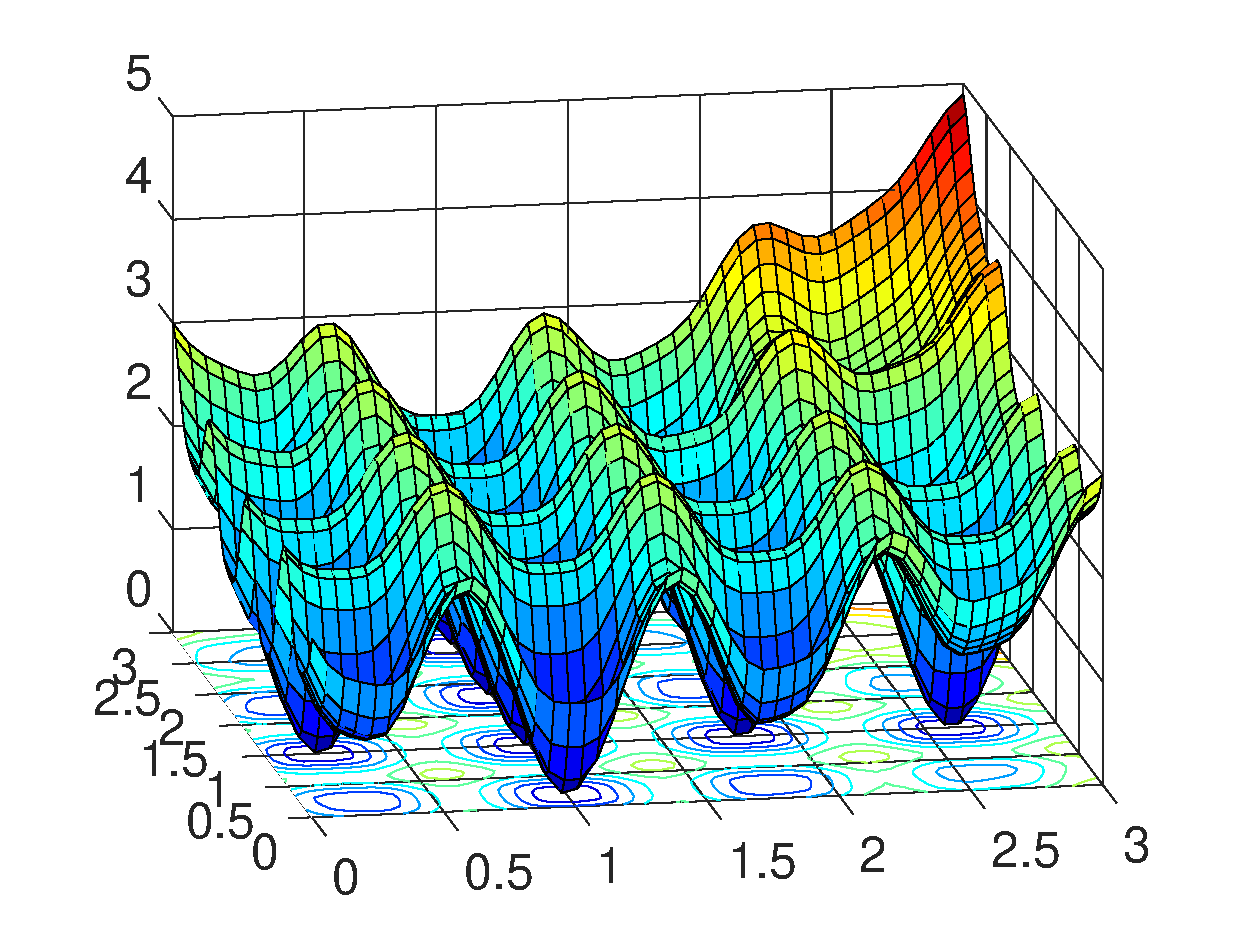
\includegraphics[width=0.98\textwidth]{chapters/minimization-fx/mfiles/fxxq3/surfcfx3.eps}
         \caption{Superfície $e(\VECTOR{x})$. }
         \label{fig:ex:minfxbCfxbaxqaxq3:a}
     \end{subfigure}
     \hfill
     \begin{subfigure}[b]{0.49\textwidth}
         \centering
         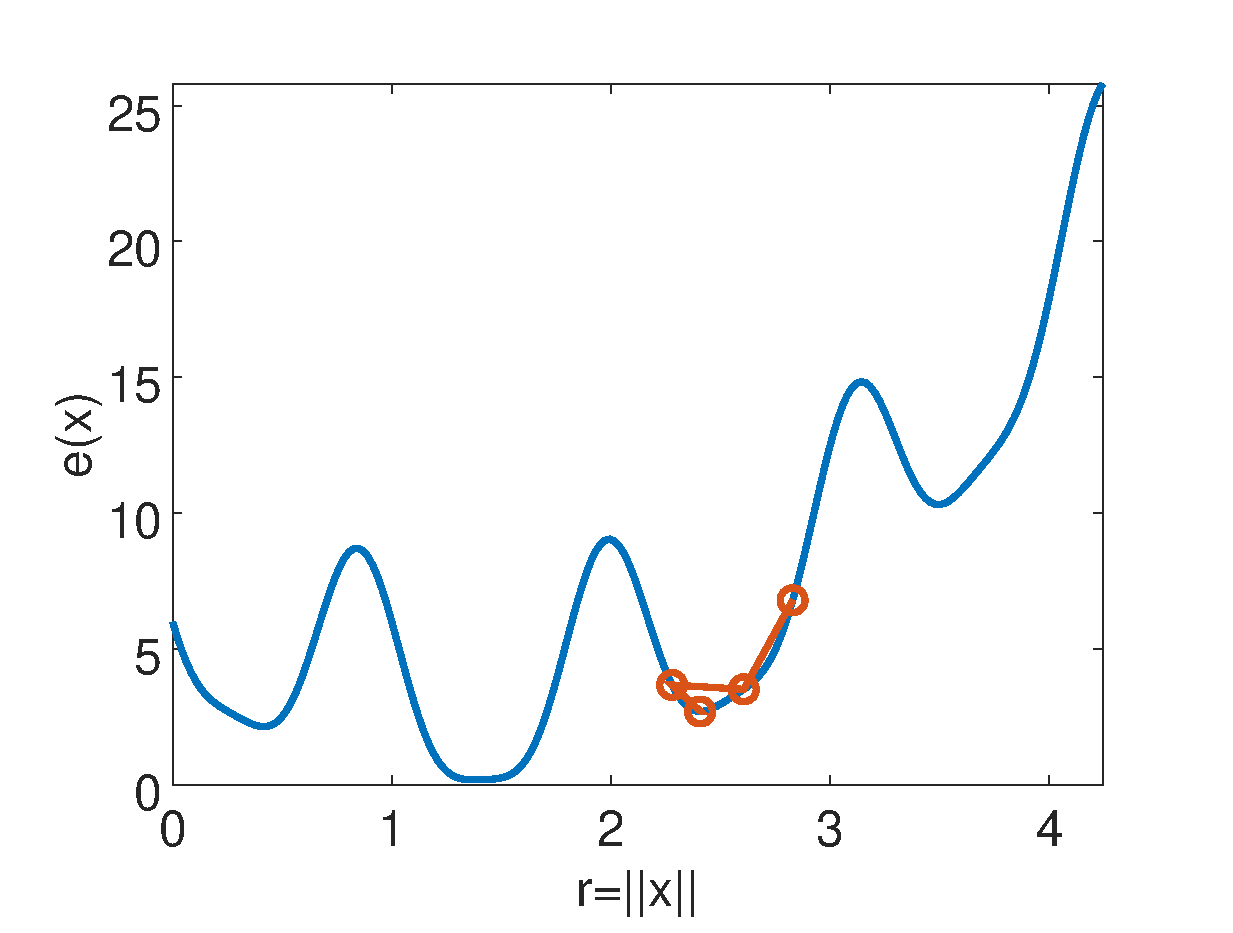
\includegraphics[width=0.98\textwidth]{chapters/minimization-fx/mfiles/fxxq3/plotfx3.eps}
         \caption{Curva $e(\VECTOR{x})$ na direção $(1,1)$.}
         \label{fig:ex:minfxbCfxbaxqaxq3:b}
     \end{subfigure}
        \caption{Resposta gráfica do Exemplo \ref{ex:minfxbCfxbaxqaxq1}. }
        \label{fig:ex:minfxbCfxbaxqaxq3}
\end{figure}

\begin{SolutionT}[Relativa ao Exemplo \ref{ex:minfxbCfxbaxqaxq1}:]
\label{ex:minfxbCfxbaxqaxq3:sol2}
Se escolhemos o ponto inicial $\VECTOR{x}_0=[\frac{11.0999}{5}$ $\frac{11.0999}{5}]^{\transpose}$,
com pendente\footnote{O cálculo da
pendente de $e(\VECTOR{\hat{x}})$ pode ser visto no Teorema \ref{theo:derfxbCfxb0}.} 
$\frac{\partial e(\VECTOR{x}_0)}{\partial \VECTOR{x} }=[0.44442\quad 0.44442]^{\transpose}$ e 
usamos iterativamente a Eq. (\ref{eq:minfxbCfxbaxqaxq2}), obtemos os valores 
$\VECTOR{x}_k$ e $e(\VECTOR{x}_k)$, como mostra a Tabela \ref{table:ex:minfxbCfxbaxqaxq4},
na qual se assume o final do processo iterativo quando $\VECTOR{x}_k \approx \VECTOR{x}_{k-1}$.
Assim, a aproximação iterativa conclui na resposta 
$\VECTOR{\hat{x}}\approx \VECTOR{x}_{7} =[0.97172\quad 0.97172]^{\transpose}$
com um erro $e(\VECTOR{\hat{x}})=0.19325$ e uma pendente
$\frac{\partial e(\VECTOR{\hat{x}})}{\partial \VECTOR{x} }=[-0.0037461\quad -0.0037461]^{\transpose}$;
esse processo pode ser visto de forma gráfica na Figura \ref{fig:ex:minfxbCfxbaxqaxq4:b}.
\end{SolutionT}


\begin{table}[h!]
\centering
\begin{tabular}{|l|l|l|l|l|l|l|l|l|}
\hline
$k$ & 0 & 1 & 2 & 3 & 4 & 5 & 6 & 7\\ \hline
$\VECTOR{x}_k$ & 2.21998 & 2.15837 & 1.27881 & 1.02790 & 0.98814 & 0.96083 & 0.97294 & 0.97172 \\ 
~              & 2.21998 & 2.15837 & 1.27881 & 1.02790 & 0.98814 & 0.96083 & 0.97294 & 0.97172 \\ \hline
$||\VECTOR{x}_k||$ & 3.1395 & 3.0524 & 1.8085 & 1.4537 & 1.3974 & 1.3588 & 1.3759 & 1.3742 \\ \hline
$e(\VECTOR{x}_k)$ & 14.84107 & 13.88071 & 5.63225 & 0.21557 & 0.19588 & 0.19518 & 0.19326 & 0.19325 \\ \hline
\end{tabular}
\caption{Resposta iterativa do Exemplo \ref{ex:minfxbCfxbaxqaxq1}.}
\label{table:ex:minfxbCfxbaxqaxq4}
\end{table}

     \begin{figure}[!h]
         \centering
         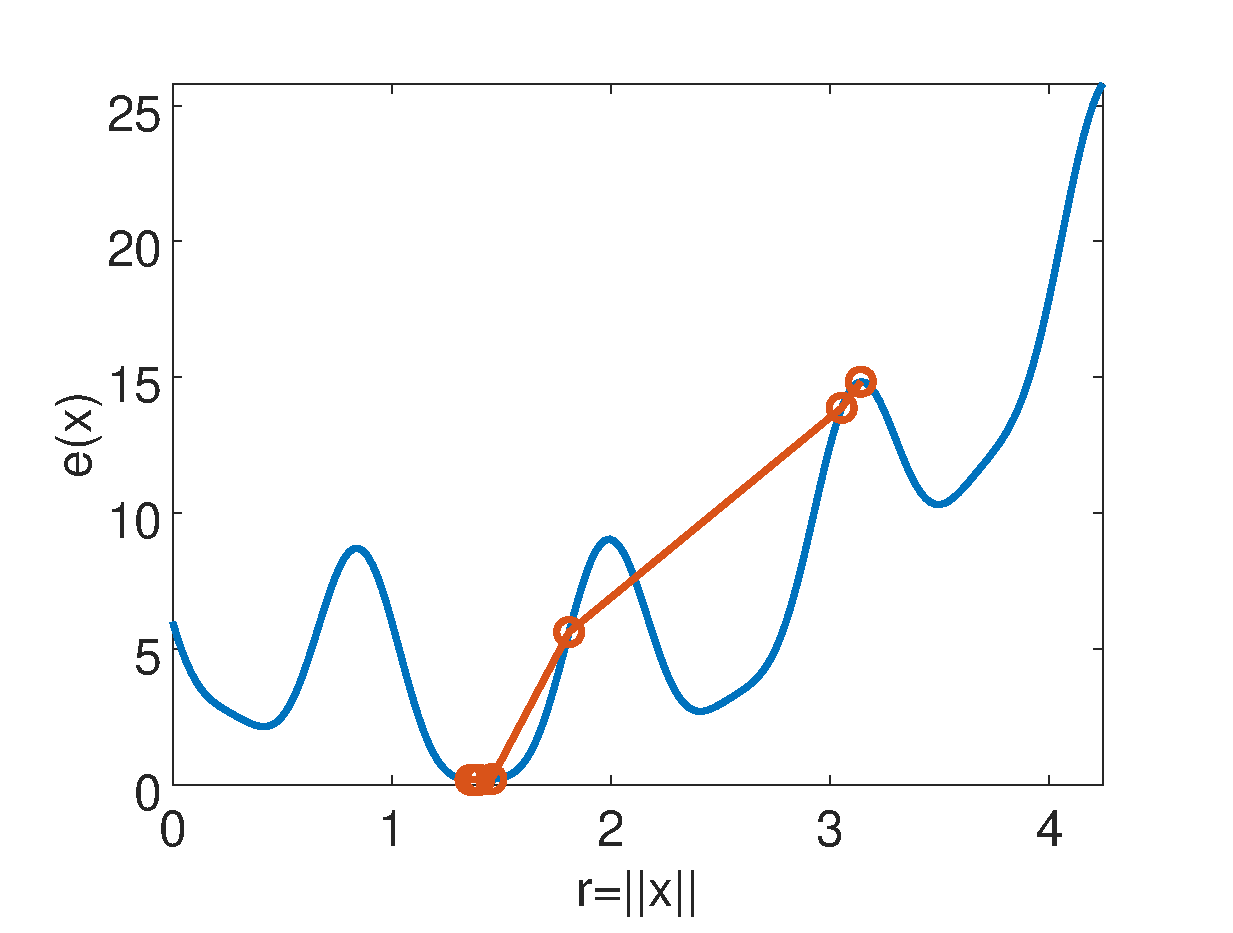
\includegraphics[width=0.5\textwidth]{chapters/minimization-fx/mfiles/fxxq3/plotfx4.eps}
         \caption{Curva $e(\VECTOR{x})$ na direção $(1,1)$.}
         \label{fig:ex:minfxbCfxbaxqaxq4:b}
     \end{figure}



\newpage

\section{Minimização de $||\VECTOR{f}(\VECTOR{x})-\VECTOR{b}||_{\MATRIX{C}}^2+\alpha||\VECTOR{x}-\VECTOR{x}_{last}||_{\MATRIX{D}}^2$}


%\index{Minimização, métodos!Regularização de}
%\index{Problema inverso!Não linear}
\index{Minimização do erro quadrático!Não linear}%!Função $||\VECTOR{f}(\VECTOR{x})-\VECTOR{b}||_{\MATRIX{C}}^2+\alpha||\VECTOR{x}-\VECTOR{x}_{last}||_{\MATRIX{D}}^2$}

\begin{theorem}[Solução iterativa]\label{theo:minfxbCfxbaxoaxo}
Dados,
o escalar $\alpha \in \mathbb{R}_{+}$,
os vetores coluna $\VECTOR{x}\in \mathbb{R}^N$, $\VECTOR{b}\in \mathbb{R}^M$ e $\VECTOR{x}_{last}\in \mathbb{R}^N$,  
uma função $\VECTOR{f}:\mathbb{R}^{N} \rightarrow \mathbb{R}^{M}$, 
as matrizes diagonais $\MATRIX{C} \in \mathbb{R}^{M\times M}_{+}$ e $\MATRIX{D} \in \mathbb{R}^{N\times N}_{+}$, e 
definida a Eq. (\ref{eq:minfxbCfxbaxoaxo1}),
\begin{equation}\label{eq:minfxbCfxbaxoaxo1}
e(\VECTOR{x})=||\VECTOR{f}(\VECTOR{x})-\VECTOR{b}||_{\MATRIX{C}}^2+\alpha||\VECTOR{x}-\VECTOR{x}_{last}||_{\MATRIX{D}}^2,
\end{equation}
onde consideramos que $\VECTOR{x}_{last}$ é uma constante equivalente a $\VECTOR{x}_{k-1}$
numa busca iterativa ou equivalente a $\VECTOR{p}$, 
se decidimos usar uma aproximação linear ao redor de $\VECTOR{p}$ em $\VECTOR{f}(\VECTOR{x})$; 
é dizer, o segundo somando na Eq. (\ref{eq:minfxbCfxbaxoaxo1}) 
procura minimizar $||\VECTOR{x}_{k}-\VECTOR{x}_{k-1}||_{\MATRIX{D}}^2$.


Se desejamos achar o ponto $\VECTOR{x}=\VECTOR{\hat{x}}$ que minimiza o escalar $e(\VECTOR{x})$,
podemos obtê-lo usando iterativamente a Eq. (\ref{eq:minfxbCfxbaxoaxo2}),
onde  $\MATRIX{J}(\VECTOR{x})$ é a \hyperref[def:jacobian]{\textbf{matriz Jacobiana}}  de $\VECTOR{f}(\VECTOR{x})$,
\begin{equation}\label{eq:minfxbCfxbaxoaxo2}
\VECTOR{x}_{k}\leftarrow \VECTOR{x}_{k-1}-
\left[ \MATRIX{J}(\VECTOR{x}_{k-1})^{\transpose}\MATRIX{C} \MATRIX{J}(\VECTOR{x}_{k-1}) +\alpha\MATRIX{D} \right]^{-1}
 \left[\MATRIX{J}(\VECTOR{x}_{k-1})^{\transpose}\MATRIX{C}\left\{\VECTOR{f}(\VECTOR{x}_{k-1})-\VECTOR{b}\right\}\right];
\end{equation}
onde em cada iteração se tenta minimizar
\begin{equation}\label{eq:minfxbCfxbaxoaxo2:ex}
e_{k-1}(\VECTOR{x})  \equiv 
||\VECTOR{f}(\VECTOR{x})-\VECTOR{b}||_{\MATRIX{C}}^2+
\alpha||\VECTOR{x}-\VECTOR{x}_{k-1}||_{\MATRIX{D}}^2.
\end{equation}
Assim, $\VECTOR{\hat{x}}$ pode ser achado 
iniciando a Eq. (\ref{eq:minfxbCfxbaxoaxo2}) desde um $\VECTOR{x}_{0}$ qualquer, 
ate que $\VECTOR{x}_{k}$ seja muito próximo a $\VECTOR{x}_{k-1}$,
onde se declara que $\VECTOR{\hat{x}} \approx \VECTOR{x}_{k}$,
que corresponde a um mínimo\footnote{\label{ref:minfxxp}A
demostração pode ser vista na Prova \ref{proof:theo:minfxbCfxbaxod}.} de $e(\VECTOR{x})$,
sem aclarar se é local ou global.


\textbf{Considerações:}

\begin{itemize}
\item É interessante verificar sempre na Eq. (\ref{eq:minfxbCfxbaxoaxo2}) 
se  $\MATRIX{J}(\VECTOR{x}_{k-1}) = \MATRIX{0}$,
pois indica que existe\footref{ref:minfxxp} um ponto de inflexão 
(máximo, mínimo ou ponto de sela) em $e(\VECTOR{x}_{k-1})$;
consequentemente poderíamos ter achado um mínimo.
\item A busca iterativa da Eq. (\ref{eq:minfxbCfxbaxoaxo2}) é considerada falida quando 
$\MATRIX{J}(\VECTOR{x}_{k-1})^{\transpose}\MATRIX{C} \MATRIX{J}(\VECTOR{x}_{k-1}) +\alpha\MATRIX{D}$
não tem inversa.
\end{itemize}


\end{theorem} 


\begin{tcbattention}
\begin{itemize}
\item O Teorema \ref{theo:minfxbCfxbaxoaxo} pode ser usado para achar o vetor $\VECTOR{x}$
que minimize $||\VECTOR{f}(\VECTOR{x})-\VECTOR{b}||_{\MATRIX{C}}^2$, procurando 
em todo momento que na busca iterativa se minimize $||\VECTOR{x}_{k}-\VECTOR{x}_{k-1}||_{\MATRIX{D}}^2$,
\end{itemize}
\end{tcbattention}

%%%%%%%%%%%%%%%%%%%%%%%%%%%%%%%%%%%%%%%%%%%%%%%%%%%%%%%%%%%%%%%%%%%%%%%%%%%%%%%%
\subsection{Exemplos de minimização de 
$||\VECTOR{f}(\VECTOR{x})-\VECTOR{b}||_{\MATRIX{C}}^2+\alpha||\VECTOR{x}-\VECTOR{x}_{last}||_{\MATRIX{D}}^2$}


\begin{example}[Quando existem muitos mínimos locais e um
$\VECTOR{\hat{x}}$ que cumpre que $\VECTOR{f}(\VECTOR{\hat{x}}) \approx \VECTOR{b}$:]
\label{ex:minfxbCfxbaxqaxp1}
Conhecida um escalar $\alpha$, uma função $\VECTOR{f}(\VECTOR{x}) : \mathbb{R}^{2} \rightarrow \mathbb{R}^{3}$,
um ponto $\VECTOR{b}$ no contradomínio de $\VECTOR{f}(\VECTOR{x})$;
achar o valor $\VECTOR{\hat{x}}$ que minimize 
$||\VECTOR{f}(\VECTOR{x})-\VECTOR{b}||_{\MATRIX{C}}^2+\alpha||\VECTOR{x}-\VECTOR{x}_{last}||_{\MATRIX{D}}^2$;
sabendo que:
\begin{equation}
\VECTOR{b}=\begin{bmatrix}
1\\
1\\
2
\end{bmatrix},
\qquad 
\VECTOR{f}(\VECTOR{x})=\begin{bmatrix}
sin(\frac{x_1 5 \pi}{2})\\
sin(\frac{x_2 5 \pi}{2})\\
x_1+x_2
\end{bmatrix},
\qquad
\alpha=0.5.
\end{equation}
Com esta informação podemos calcular o jacobiano $\MATRIX{J}(\VECTOR{x})$ de $\VECTOR{f}(\VECTOR{x})$,
 e também escolher as matrizes $\MATRIX{C} \in \mathbb{R}^{3}$ e $\MATRIX{D} \in \mathbb{R}^{2}$, 
com elementos iguais à  matriz identidade. 
Assim, usando a Eq. (\ref{eq:minfxbCfxbaxoaxo2:ex}),
obtemos a superfície $e_{0}(\VECTOR{x})$ para um ponto inicial $\VECTOR{x}_0$ como mostra a Figura \ref{fig:ex:minfxbCfxbaxqaxp3:a}.
Podemos ver a resposta a este exemplo na Solução \ref{ex:minfxbCfxbaxqaxp3:sol1}.
\end{example}

\begin{SolutionT}[Relativa ao Exemplo \ref{ex:minfxbCfxbaxqaxp1}:]
\label{ex:minfxbCfxbaxqaxp3:sol1}
Se escolhemos o ponto inicial $\VECTOR{x}_0=[2.2183$ $2.2183]^{\transpose}$ e 
usamos iterativamente a Eq. (\ref{eq:minfxbCfxbaxoaxo2}), obtemos os valores 
de $\VECTOR{x}_k$ e $e_{k}(\VECTOR{x}_k)$, como mostra a Tabela \ref{table:ex:minfxbCfxbaxqaxp3},
onde se assume o final do processo iterativo quando $\VECTOR{x}_k \approx \VECTOR{x}_{k-1}$.
Assim, a aproximação iterativa conclui na resposta 
$\VECTOR{\hat{x}}\approx \VECTOR{x}_{4} =[1.0304\quad 1.0304]^{\transpose}$
com um erro $e_{4}(\VECTOR{\hat{x}})=6.6750~10^{-3}$;
este processo pode ser visto de forma gráfica na Figura \ref{fig:ex:minfxbCfxbaxqaxp3:b}.
\end{SolutionT}

\begin{table}[h!]
\centering
\begin{tabular}{|l|l|l|l|l|l|}
\hline
$k$ & 0 & 1 & 2 & 3 & 4 \\ \hline
$\VECTOR{x}_k$ & 2.2183 & 2.1656 & 1.2297 & 1.0676 & 1.0304 \\ 
~              & 2.2183 & 2.1656 & 1.2297 & 1.0676 & 1.0304 \\ \hline
$||\VECTOR{x}_k||$ & 3.1371 & 3.0627 & 1.7391 & 1.5099 & 1.4571 \\ \hline
$e_{k}(\VECTOR{x}_k)$ & 1.3855e+01 & 1.3151e+01 & 4.1187e+00 & 8.2579e-02 & 6.6750e-03 \\ \hline
\end{tabular}
\caption{Resposta iterativa do Exemplo \ref{ex:minfxbCfxbaxqaxp1}.}
\label{table:ex:minfxbCfxbaxqaxp3}
\end{table}
\begin{figure}[h!]
     \centering
     \begin{subfigure}[b]{0.49\textwidth}
         \centering
         \includegraphics[width=0.98\textwidth]{chapters/minimization-fx/mfiles/fxxx3/surfcfx3-0.eps}
         \caption{Superfície $e_0(\VECTOR{x})$.}
         \label{fig:ex:minfxbCfxbaxqaxp3:a}
     \end{subfigure}
     \hfill
     \begin{subfigure}[b]{0.49\textwidth}
         \centering
         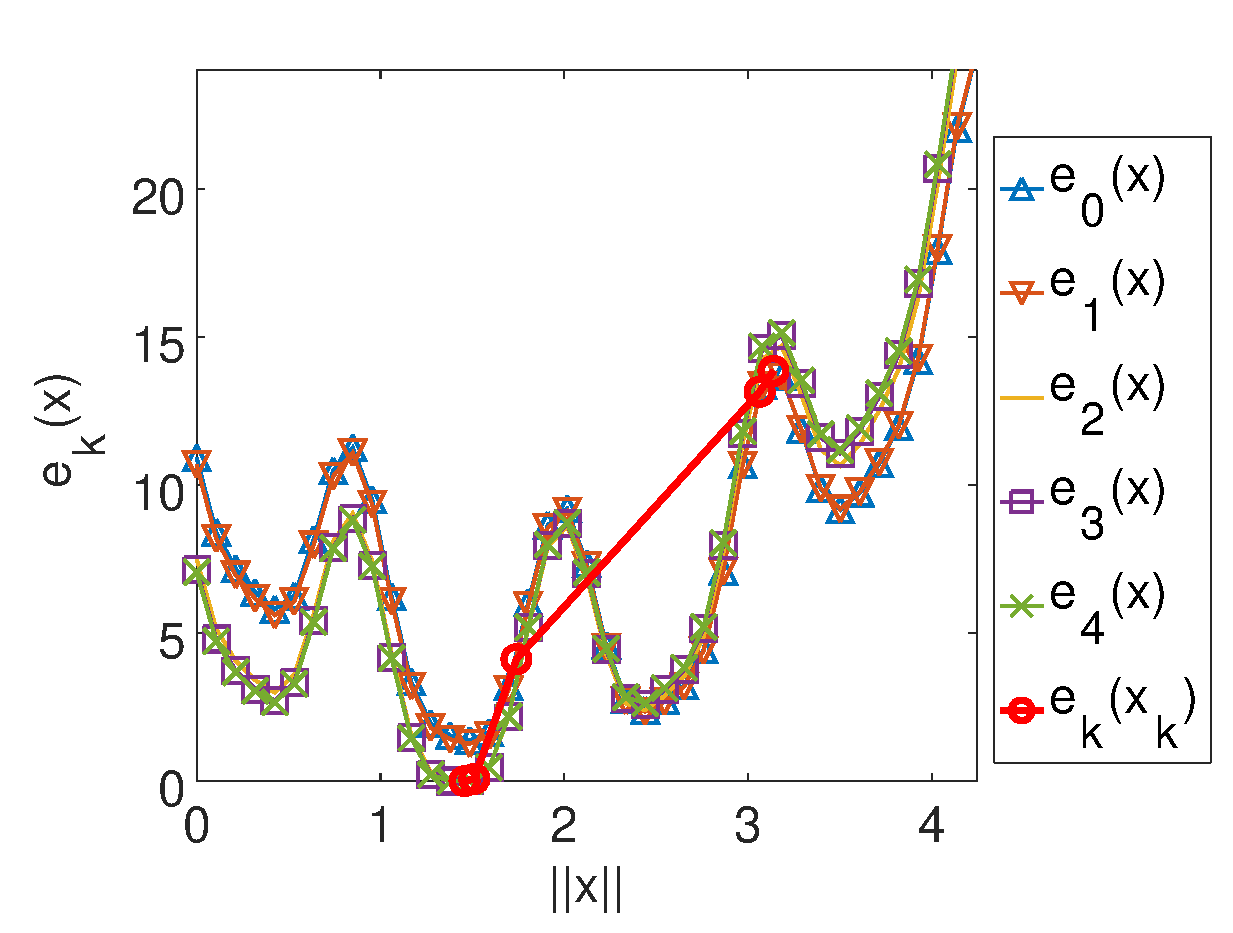
\includegraphics[width=0.98\textwidth]{chapters/minimization-fx/mfiles/fxxx3/plotfx3all.eps}
         \caption{Curva $e(\VECTOR{x})$ na direção $(1,1)$.}
         \label{fig:ex:minfxbCfxbaxqaxp3:b}
     \end{subfigure}
        \caption{Resposta gráfica do Exemplo \ref{ex:minfxbCfxbaxqaxp1}. }
        \label{fig:ex:minfxbCfxbaxqaxp3}
\end{figure}



\newpage



\begin{comment}
%%%%%%%%%%%%%%%%%%%%%%%%%%%%%%%%%%%%%%%%%%%%%%%%%%%%%%%%%%%%%%%%%%%%%%%%%%%%%%%%%%%%%%%
\section{Minimização de $\frac{||\VECTOR{f}(\VECTOR{x})-\VECTOR{b}||^2}{||\VECTOR{b}||^2}$
$+\alpha\frac{||\VECTOR{x}-\VECTOR{q}||^2}{||\VECTOR{q}||^2}$  
}
\textcolor{red}{Inventado por mi ..., creo.}
%%%%%%%%%%%%%%%%%%%%%%%%%%%%%%%%%%%%%%%%%%%%%%%%%%%%%%%%%%%%%%%%%%%%%%%%%%%%%%%%%%%%%%%
\section{Minimização de $||\VECTOR{f}(\VECTOR{x})-\VECTOR{b}||_{\MATRIX{B}^{-2}}^2$
$+\alpha||\VECTOR{x}-\VECTOR{q}||_{\MATRIX{Q}^{-2}}^2$  
}
\textcolor{red}{Inventado por mi ..., creo Nenhun valor de $\VECTOR{b}$ ou $\VECTOR{q}$ pode ser zero.}
\end{comment}

